
\documentclass[12pt,a4paper]{report}

% Packages
\usepackage[a4paper,left=20mm,right=20mm,top=26mm,bottom=32mm,includeheadfoot,headheight=28pt,headsep=8mm,footskip=18mm]{geometry}
\usepackage{graphicx}
\usepackage{amsmath}
\usepackage{amssymb}
\usepackage{booktabs}
\usepackage{array}
\usepackage{tabularx}
\usepackage{float}
\usepackage{fancyhdr}
\usepackage[hidelinks]{hyperref}
\usepackage{xcolor}
\usepackage{setspace}
\usepackage{enumitem}
\usepackage{caption}

\captionsetup{
    labelfont=bf,
    justification=raggedright,
    singlelinecheck=false,
    format=plain
}
\usepackage{subcaption}
\usepackage{multirow}
\usepackage{colortbl}
\usepackage{longtable}
\setlength{\LTleft}{\fill}
\setlength{\LTright}{\fill}
\usepackage{titlesec}
\usepackage{titletoc}
\usepackage{lastpage}
\usepackage{makecell}
\usepackage{etoolbox}
\usepackage{needspace}

\numberwithin{table}{chapter}
\numberwithin{figure}{chapter}
% Table layout and spacing: consistent padding, row height, and longtable pre/post skips
\setlength{\tabcolsep}{3pt}
\renewcommand{\arraystretch}{1.12}
\setlength{\LTpre}{0pt}
\setlength{\LTpost}{6pt}
% Table rules (outline thickness) and small extra row height for clarity
\setlength{\arrayrulewidth}{0.5pt}
\setlength{\extrarowheight}{0.6pt}

% Prevent tables from overflowing past the page bottom:
% if fewer than 7 baseline-skips remain, break to the next page first.
\BeforeBeginEnvironment{table}{\Needspace{7\baselineskip}}
\BeforeBeginEnvironment{longtable}{\Needspace{7\baselineskip}}

\definecolor{osdagGreen}{HTML}{91B014}
\definecolor{reportPass}{HTML}{688510}
\definecolor{reportFail}{HTML}{C43C39}
\definecolor{reportInfo}{HTML}{245A81}
\definecolor{reportMissing}{HTML}{777777}
\newcommand{\ReportSectionStyle}{\small\setlength{\tabcolsep}{3pt}\renewcommand{\arraystretch}{1.15}}
\newcommand{\ReportCompactTable}{\setlength{\tabcolsep}{2pt}}
\newcommand{\ReportCaptionStyle}{\setlength{\abovecaptionskip}{2pt}\setlength{\belowcaptionskip}{2pt}}
\newcommand{\ReportWideRows}{\renewcommand{\arraystretch}{1.25}}

\newcommand{\ReportBrandFont}{\Huge}
\newcommand{\ReportCoverTopSpace}{\vspace*{1.5cm}}
\newcommand{\ReportTableGap}{\vspace{1em}}
\newcommand{\ReportMinorGap}{\vspace{0.4em}}
\newcommand{\ReportSectionGap}{\vspace{1.5em}}
\newcommand{\ReportMajorGap}{\vspace{2em}}
% Extra space after a table row (\\[\ReportRowGap]) and inside multi-line cells
\newlength{\ReportRowGap}\setlength{\ReportRowGap}{6pt}
\newlength{\ReportRowGapLarge}\setlength{\ReportRowGapLarge}{8pt}
\newlength{\ReportCellLineGap}\setlength{\ReportCellLineGap}{3pt}
\newlength{\ReportTitleLineGap}\setlength{\ReportTitleLineGap}{0.3cm}
\newlength{\ReportTitleBlockGap}\setlength{\ReportTitleBlockGap}{1.5cm}
\newlength{\ReportTitleLogoGap}\setlength{\ReportTitleLogoGap}{1cm}
% Check status labels
\newcommand{\ReportPass}{PASS}
\newcommand{\ReportFail}{\textcolor{reportFail}{FAIL}}
% Page-break notices for long tables (added to every longtable by continued_tables)
\newcommand{\ReportContinuedFromNumbered}{\ReportFootnoteFont\textit{\tablename~\thetable{} continued from previous page}}
\newcommand{\ReportContinuedFrom}{\ReportFootnoteFont\textit{Continued from previous page}}
\newcommand{\ReportContinuedOn}{\ReportFootnoteFont\textit{Continued on next page}}
\newcommand{\ReportSmallFont}{\small}
\newcommand{\ReportFootnoteFont}{\footnotesize}
\newcommand{\ReportNormalFont}{\normalsize}
\newcommand{\ReportLargeFont}{\large}
\newcommand{\ReportHeadingFont}{\Large}
\newcommand{\ReportTableLeft}{\setlength{\LTleft}{0pt}\setlength{\LTright}{\fill}}

\fancypagestyle{main}{
  \fancyhf{}
  \fancyhead[L]{FOSSEE report validation — 20 m bridge $|$ FOSSEE-WI-2026}
  \fancyhead[R]{2026-11-20 $|$ Rev 0}
  \fancyfoot[L]{\scriptsize Osdag $|$ FOSSEE $|$ Indian Institute of Technology Bombay}
  \fancyfoot[R]{\scriptsize Page \thepage\ of \pageref{LastPage}}
  \renewcommand{\headrule}{\color{osdagGreen}\hrule width\headwidth height 1pt \vspace{2pt}}
  \renewcommand{\footrule}{%
    \ifbool{hasSDonPage}{%
      \vspace{0pt}%
      \hbox to \headwidth{\textcolor{black}{\footnotesize\textit{* Software default value}}\hfil}%
      \vspace{4pt}%
    }{%
      \vspace{0pt}%
    }%
    \color{osdagGreen}\hrule width\headwidth height 1pt \vspace{6pt}%
  }
}
\fancypagestyle{plain}{
  \fancyhf{}
  \fancyhead[L]{FOSSEE report validation — 20 m bridge $|$ FOSSEE-WI-2026}
  \fancyhead[R]{2026-11-20 $|$ Rev 0}
  \fancyfoot[L]{\scriptsize Osdag $|$ FOSSEE $|$ Indian Institute of Technology Bombay}
  \fancyfoot[R]{\scriptsize Page \thepage\ of \pageref{LastPage}}
  \renewcommand{\headrule}{\color{osdagGreen}\hrule width\headwidth height 1pt \vspace{2pt}}
  \renewcommand{\footrule}{%
    \ifbool{hasSDonPage}{%
      \vspace{0pt}%
      \hbox to \headwidth{\textcolor{black}{\footnotesize\textit{* Software default value}}\hfil}%
      \vspace{4pt}%
    }{%
      \vspace{0pt}%
    }%
    \color{osdagGreen}\hrule width\headwidth height 1pt \vspace{6pt}%
  }
}
\fancypagestyle{firstpage}{
  \fancyhf{}
  \renewcommand{\headrulewidth}{0pt}
  \fancyfoot[L]{\scriptsize Osdag $|$ FOSSEE $|$ Indian Institute of Technology Bombay}
  \fancyfoot[R]{\scriptsize Page \thepage\ of \pageref{LastPage}}
  \renewcommand{\footrule}{\vspace{0pt}\color{osdagGreen}\hrule width\headwidth height 1pt \vspace{6pt}}
}
\pagestyle{main}
\setstretch{1.15}
\setlength{\emergencystretch}{2em}

% Custom Commands
\newcommand{\placeholder}[1]{\textit{\textless #1\textgreater}}
\newcommand{\todo}[1]{\colorbox{yellow}{TODO: #1}}
\newcolumntype{L}[1]{>{\raggedright\arraybackslash}p{#1}}
\newcolumntype{C}[1]{>{\centering\arraybackslash}p{#1}}
\newcolumntype{R}[1]{>{\raggedleft\arraybackslash}p{#1}}

% Software-default asterisk
\newcommand{\sdstar}{\textsuperscript{*}}
\newbool{hasSDonPage}
\boolfalse{hasSDonPage}
\newcommand{\markSD}{\global\booltrue{hasSDonPage}}
\renewcommand{\sdstar}{\textsuperscript{*}\markSD{}}
\AddToHook{shipout/before}{\global\boolfalse{hasSDonPage}}

\title{\Large\textbf{OsdagBridge} \\ \normalsize Open Source Software for Steel Girder Bridge Design \\ \vspace{2cm} \large Design Report}
\author{}
\date{}

% Chapter / TOC Formatting
\titleformat{\chapter}[block]
  {\normalfont\Large\bfseries\centering}{\thechapter}{1em}{}
\titlespacing*{\chapter}{0pt}{0pt}{10pt}
\setcounter{tocdepth}{2}

\begin{document}


\begin{titlepage}
\thispagestyle{firstpage}
\centering
\ReportCoverTopSpace
\noindent
\begin{minipage}[c]{0.6\textwidth}
\raggedright

\includegraphics[width=\linewidth,keepaspectratio]{Report_After_assets/osdag_logo.png}
\end{minipage}%
\hfill
\begin{minipage}[c]{0.35\textwidth}
\raggedleft

\end{minipage}
\\[\ReportTitleLogoGap]

{\ReportBrandFont \textbf{OsdagBridge}}\\[\ReportTitleLineGap]
{\ReportLargeFont Open Source Software for Steel Girder Bridge Design}\\[\ReportTitleBlockGap]
{\ReportHeadingFont Design Report}\\[\ReportTitleBlockGap]
\begin{tabular}{|L{4cm}|L{10cm}|}
\hline
\textbf{Project Name} & FOSSEE report validation — 20 m bridge \\
\hline
\textbf{Project Location} & Ahmednagar, Maharashtra \\
\hline
\textbf{Author / Designer} & Disguised18 \\
\hline
\textbf{Reviewer} &  \\
\hline
\textbf{Organization} & FOSSEE applicant \\
\hline
\textbf{Client Name and Organization} & Screening task demonstration \\
\hline
\textbf{Job Number} & FOSSEE-WI-2026 \\
\hline
\textbf{Date} & 2026-11-20 \\
\hline
\textbf{Report Version} &  \\
\hline
\end{tabular}
\end{titlepage}



% TOC styling using titletoc
\titlecontents{chapter}[1.5em]
  {\normalfont\vspace{2pt}}
  {\contentslabel{1.5em}}
  {\hspace*{-1.5em}}
  {\hfill\contentspage}

\titlecontents{section}[3.8em]
  {\normalfont}
  {\contentslabel{2.3em}}
  {\hspace*{-2.3em}}
  {\hfill\contentspage}

\titlecontents{subsection}[7.0em]
  {\normalfont}
  {\contentslabel{3.2em}}
  {\hspace*{-3.2em}}
  {\hfill\contentspage}

\newpage
\renewcommand{\contentsname}{\centering\Large\bfseries Table of Contents}
\tableofcontents

\ReportSectionStyle

\newpage
{\centering\ReportHeadingFont\bfseries Executive Summary\par}
\addcontentsline{toc}{chapter}{Executive Summary}
\ReportTableGap

This section provides a concise summary of the bridge design, key inputs, governing loads, and final design outcomes.

\section*{Project Overview}
\addcontentsline{toc}{section}{Project Overview}
\label{sec:project-overview}


\begin{longtable}{|L{5.5cm}|L{8.5cm}|}
\hline
\textbf{Parameter} & \textbf{Value} \\
\hline
\endfirsthead
\multicolumn{2}{@{}l}{\ReportContinuedFrom}\\
\hline
\textbf{Parameter} & \textbf{Value} \\
\hline
\endhead
\noalign{\vskip-\arrayrulewidth}\hline
\multicolumn{2}{@{}r@{}}{\ReportContinuedOn}\\
\endfoot
\endlastfoot
\textbf{Bridge Type} & Highway Bridge \\
\hline
\textbf{Design Standard} & IRC 5, IRC 6, IRC 22, IRC 24, IS 800 \\
\hline
\textbf{Span} & 20 m \\
\hline
\textbf{Carriageway Width} & 7.5 m \\
\hline
\textbf{No. of Girders} & 5 \\
\hline
\textbf{Girder Spacing} & 2.43 \\
\hline
\textbf{Deck Thickness} & 250.0 \\
\hline
\textbf{Overall Design Status} & Fail (Fatigue Normal Stress, Fatigue Shear Stress) \\
\hline
\textbf{Governing Check} & Fatigue Normal Stress \\
\hline
\textbf{Overall Utilization Ratio (max)} & 2.56 (Girder) \\
\hline
\end{longtable}


\begin{figure}[H]
\centering
\fbox{\parbox{0.97\textwidth}{
\textit{[ PLACEHOLDER: Figure 1 -- Overall Bridge Plan ]}
}}
\caption*{Figure 1 -- Overall Bridge Plan}
\end{figure}

\newpage

\begin{figure}[H]
\centering
\fbox{\parbox{0.97\textwidth}{
\textit{[ PLACEHOLDER: Figure 2 -- Typical Cross-Section (with girder, deck, barriers, footpath) ]}
}}
\caption*{Figure 2 -- Typical Cross-Section (with girder, deck, barriers, footpath)}
\end{figure}

\begin{figure}[H]
\centering
\fbox{\parbox{0.97\textwidth}{
\textit{[ PLACEHOLDER: Figure 3 -- 3D View of Bridge Superstructure ]}
}}
\caption*{Figure 3 -- 3D View of Bridge Superstructure}
\end{figure}

\noindent\textbf{Table 1 -- Final Bridge Geometry (after optimization)}

\ReportMinorGap
\noindent
\begin{longtable}{|C{2.8cm}|C{2.4cm}|C{2.4cm}|C{2.4cm}|C{2.4cm}|C{2.4cm}|}
\hline
  \textbf{} &
  \textbf{G1} &
  \textbf{G2} &
  \textbf{G3} &
  \textbf{G4} &
  \textbf{G5} \\
\hline
\endfirsthead
\multicolumn{6}{@{}l}{\ReportContinuedFrom}\\
\hline
  \textbf{} &
  \textbf{G1} &
  \textbf{G2} &
  \textbf{G3} &
  \textbf{G4} &
  \textbf{G5} \\
\hline
\endhead
\noalign{\vskip-\arrayrulewidth}\hline
\multicolumn{6}{@{}r@{}}{\ReportContinuedOn}\\
\endfoot
\endlastfoot
Member ID & G1M1 & G2M1 & G3M1 & G4M1 & G5M1 \\
\hline
Section Designation & 1120 x 340 x 16 x 340 x 16 & 1120 x 340 x 16 x 340 x 16 & 1120 x 340 x 16 x 340 x 16 & 1120 x 340 x 16 x 340 x 16 & 1120 x 340 x 16 x 340 x 16 \\
\hline
Governing Check & Fatigue Normal Stress & Fatigue Normal Stress & Fatigue Normal Stress & Fatigue Normal Stress & Fatigue Normal Stress \\
\hline
Utilization Ratio & 2.56 (Girder) & 2.56 (Girder) & 2.56 (Girder) & 2.56 (Girder) & 2.56 (Girder) \\
\hline
\end{longtable}

\ReportMinorGap
\noindent\textit{Note: Utilization ratio (UR) = demand / capacity. A value $< 1.0$ indicates a passing check.}

\ReportTableGap

\section*{Key Design Outcomes Summary}
\addcontentsline{toc}{section}{Key Design Outcomes Summary}
\label{sec:key-outcomes}

\noindent Girder design pass \\
Cross bracing design pass \\
End Diaphragm design pass \\
Deck design pass

\section*{Design Assumptions and Limitations}
\addcontentsline{toc}{section}{Design Assumptions and Limitations}
\label{sec:assumptions}

\begin{itemize}
\item Additional inputs not provided by the user were assumed by software per IRC/IS code defaults or practical consideration.
\item Grillage analysis was performed using OSPGrillage assuming simply supported I-girders.
\item Substructure and foundation design are not included in this report.
\item Splice connections and bearings are not designed in this version.
\end{itemize}

% Restore numbered chapter format
\titleformat{\chapter}[block]{\normalfont\ReportHeadingFont\bfseries\centering}{\thechapter}{1em}{}
\titlespacing*{\chapter}{0pt}{-30pt}{10pt}

\ReportSectionStyle

\chapter{Project Information}

This section records all project metadata as entered by the designer.

\section{Project and Design Team Details}
\label{sec:project-details}

\begin{longtable}{|L{5.5cm}|L{8.5cm}|}
\hline
\textbf{Parameter} & \textbf{Value} \\
\hline
\endfirsthead
\multicolumn{2}{@{}l}{\ReportContinuedFrom}\\
\hline
\textbf{Parameter} & \textbf{Value} \\
\hline
\endhead
\noalign{\vskip-\arrayrulewidth}\hline
\multicolumn{2}{@{}r@{}}{\ReportContinuedOn}\\
\endfoot
\endlastfoot

\textbf{Project Name} & FOSSEE report validation — 20 m bridge \\
\hline
\textbf{Project Location} & Ahmednagar, Maharashtra \\
\hline
\textbf{Designer} & Disguised18 \\
\hline
\textbf{Reviewer} &  \\
\hline
\textbf{Organization} & FOSSEE applicant \\
\hline
\textbf{Client} & Screening task demonstration \\
\hline
\textbf{Software Version} & OsdagBridge \\
\hline
\end{longtable}


\section{Applicable Codes and Standards}
\label{sec:codes}

\begin{itemize}
\item Indian Roads Congress (IRC) 5: General Features of Design
\item Indian Roads Congress (IRC) 6: Loads and Load Combinations
\item Indian Roads Congress (IRC) 22: Composite Construction (Limit State Design)
\item Indian Roads Congress (IRC) 24: Steel Road Bridges (Limit State Method)
\item Indian Roads Congress (IRC) 112: Concrete Road Bridges (deck design)
\item Indian Roads Congress Special Publication (IRC SP) 114: Seismic Design of Road Bridges
\item Indian Standard (IS) 800: General Construction in Steel
\item Indian Standard (IS) 2062: Hot Rolled Structural Steel Specification
\item Indian Standard (IS) 6006: Steel Bearings
\end{itemize}

\ReportSectionStyle

\chapter{Input Parameters}

\ReportCaptionStyle

This section documents all inputs provided to OsdagBridge. User-provided inputs are clearly distinguished from software-assumed defaults. Where the user did not supply a value, the software has applied the IRC/IS code default or an empirical guideline; these are annotated with an asterisk (\sdstar{}).

\section{Basic Inputs (User-Defined)}
\label{sec:basic-inputs}

\noindent\textit{Note: These inputs are mandatory and were provided by the user.}

\begin{longtable}{|L{5.5cm}|L{8.5cm}|}

\caption{\textbf{Project Location}}
\label{subsec:project-location}\\
\hline
\textbf{Parameter} & \textbf{Value} \\
\hline
\endfirsthead
\multicolumn{2}{@{}l}{\ReportContinuedFromNumbered}\\
\hline
\textbf{Parameter} & \textbf{Value} \\
\hline
\endhead
\noalign{\vskip-\arrayrulewidth}\hline
\multicolumn{2}{@{}r@{}}{\ReportContinuedOn}\\
\endfoot
\endlastfoot

\textnormal{Project Location} & Ahmednagar, Maharashtra \\
\hline
\textnormal{Latitude / Longitude} & 19.0948, 74.748 \\
\hline
\textnormal{Seismic Zone (IRC 6)} &  \\
\hline
\textnormal{Basic Wind Speed (IRC 6)} &  \\
\hline
\textnormal{Shade Temp. Max / Min (IRC 6)} & 48.2 °C / 2.2 °C \\
\hline
\end{longtable}
\ReportTableGap


\begin{longtable}{|L{5.5cm}|L{8.5cm}|}

\caption{\textbf{Bridge Geometry}}
\label{subsec:bridge-geometry}\\
\hline
\textbf{Parameter} & \textbf{Value} \\
\hline
\endfirsthead
\multicolumn{2}{@{}l}{\ReportContinuedFromNumbered}\\
\hline
\textbf{Parameter} & \textbf{Value} \\
\hline
\endhead
\noalign{\vskip-\arrayrulewidth}\hline
\multicolumn{2}{@{}r@{}}{\ReportContinuedOn}\\
\endfoot
\endlastfoot

\textnormal{Type of Structure} & Highway Bridge \\
\hline
\textnormal{Span (m)} & 20 m \\
\hline
\textnormal{Carriageway Width (m)} & 7.5 m \\
\hline
\textnormal{Include Median} & No \\
\hline
\textnormal{Footpath} & Both Sides \\
\hline
\textnormal{Skew Angle (degrees)} & 0° (IRC 24 Cl. 504.8 limit: $\pm$15°) \\
\hline
\end{longtable}

\ReportTableGap

\begin{longtable}{|L{5.5cm}|L{8.5cm}|}

\caption{\textbf{Material Selection}}
\label{subsec:material}\\
\hline
\textbf{Parameter} & \textbf{Value} \\
\hline
\endfirsthead
\multicolumn{2}{@{}l}{\ReportContinuedFromNumbered}\\
\hline
\textbf{Parameter} & \textbf{Value} \\
\hline
\endhead
\noalign{\vskip-\arrayrulewidth}\hline
\multicolumn{2}{@{}r@{}}{\ReportContinuedOn}\\
\endfoot
\endlastfoot

\textnormal{Girder Steel Grade (IS 2062)} & E 350A \\
\hline
\textnormal{Cross Bracing Steel Grade} & E 350A \\
\hline
\textnormal{End Diaphragm Steel Grade} & E 350A \\
\hline
\textnormal{Concrete Deck Grade (IRC 22)} & M40 \\
\hline
\end{longtable}

\ReportTableGap

\newpage
\section{Additional Inputs}
\label{sec:additional-inputs}

Where the user has modified additional inputs, those values are reported here. Where no modification was made, the software default is shown.

\ReportSectionGap

\begin{longtable}{|L{5.5cm}|p{10.0cm}|}
\caption{\textbf{Typical Section Details}}\\
\hline
\textbf{Parameter} & \textbf{Value} \\
\hline
\endfirsthead
\multicolumn{2}{@{}l}{\ReportContinuedFromNumbered}\\
\hline
\textbf{Parameter} & \textbf{Value} \\
\hline
\endhead
\noalign{\vskip-\arrayrulewidth}\hline
\multicolumn{2}{@{}r@{}}{\ReportContinuedOn}\\
\endfoot
\endlastfoot

\textnormal{Overall Bridge Width (m)} & 12.149999999999999 \\[\ReportRowGap]
\hline
\textnormal{No. of Girders} & 5 \\[\ReportRowGap]
\hline
\textnormal{Girder Spacing (m)} & 2.43 m \\[\ReportRowGap]
\hline
\textnormal{Deck Overhang Width (m)} & 1.215 m \\[\ReportRowGap]
\hline
\textnormal{Deck Thickness (mm)} & 250.0 mm \\[\ReportRowGap]
\hline
\textnormal{Footpath Width (m)} & 1.5 m (IRC 5 Cl. 104.3.6 min: 1.5 m) \\[\ReportRowGap]
\hline
\textnormal{No. of Traffic Lanes} &  (per IRC 5 Cl. 104.3.1) \\[\ReportRowGap]
\hline
\end{longtable}

\ReportTableGap

\begin{longtable}{|L{5.5cm}|p{10.0cm}|}
\caption{\textbf{Components Details}}\\
\hline
\textbf{Parameter} & \textbf{Value} \\
\hline
\endfirsthead
\multicolumn{2}{@{}l}{\ReportContinuedFromNumbered}\\
\hline
\textbf{Parameter} & \textbf{Value} \\
\hline
\endhead
\noalign{\vskip-\arrayrulewidth}\hline
\multicolumn{2}{@{}r@{}}{\ReportContinuedOn}\\
\endfoot
\endlastfoot

\textnormal{Crash Barrier Type} & IRC 5 - RCC Crash Barrier \\[\ReportRowGap]
\hline
\textnormal{Crash Barrier Load (kN/m)} & 7.557 \\[\ReportRowGap]
\hline

\textnormal{Railing Type} & IRC 5 - RCC Railing \\[\ReportRowGap]
\hline
\textnormal{Railing Load (kN/m)} & 1.4715 \\[\ReportRowGap]
\hline
\textnormal{Wearing Course Material} & Concrete \\[\ReportRowGap]
\hline
\textnormal{Wearing Course Thickness (mm)} & 50.0 mm \\[\ReportRowGap]
\hline
\end{longtable}


\newpage

\ReportMinorGap
\noindent

\ReportMinorGap
\begin{longtable}{|L{2.2cm}|L{1.8cm}|p{3.8cm}|p{3.8cm}|p{3.8cm}|}
\caption{\textbf{Girder General Information}}\\
\hline
\textbf{Girder} & \textbf{Member ID} & \textbf{Design Mode} & \textbf{Girder Type} & \textbf{Girder Symmetry} \\[\ReportRowGap]
\hline
\endfirsthead
\multicolumn{5}{@{}l}{\ReportContinuedFromNumbered}\\
\hline
\textbf{Girder} & \textbf{Member ID} & \textbf{Design Mode} & \textbf{Girder Type} & \textbf{Girder Symmetry} \\[\ReportRowGap]
\hline
\endhead
\noalign{\vskip-\arrayrulewidth}\hline
\multicolumn{5}{@{}r@{}}{\ReportContinuedOn}\\
\endfoot
\endlastfoot

G1 & G1M1 & Optimized & Welded & Girder Symmetric \\[\ReportRowGapLarge]
\hline
G2 & G2M1 & Optimized & Welded & Girder Symmetric \\[\ReportRowGapLarge]
\hline
G3 & G3M1 & Optimized & Welded & Girder Symmetric \\[\ReportRowGapLarge]
\hline
G4 & G4M1 & Optimized & Welded & Girder Symmetric \\[\ReportRowGapLarge]
\hline
G5 & G5M1 & Optimized & Welded & Girder Symmetric \\[\ReportRowGapLarge]
\hline
\end{longtable}

\ReportMinorGap

\ReportMinorGap
\begin{longtable}{|L{1.8cm}|L{2.3cm}|L{1.8cm}|p{4.8cm}|p{4.8cm}|}
\caption{\textbf{Girder Section Dimensions}}\\
\hline
\textbf{Girder} & \textbf{Total Depth, D (mm)} & \textbf{Web, $t_w$ (mm)} & \textbf{Top Flange (b\textsubscript{tf}, t\textsubscript{tf}) mm} & \textbf{Bottom Flange (b\textsubscript{bf}, t\textsubscript{bf}) mm} \\[\ReportRowGap]
\hline
\endfirsthead
\multicolumn{5}{@{}l}{\ReportContinuedFromNumbered}\\
\hline
\textbf{Girder} & \textbf{Total Depth, D (mm)} & \textbf{Web, $t_w$ (mm)} & \textbf{Top Flange (b\textsubscript{tf}, t\textsubscript{tf}) mm} & \textbf{Bottom Flange (b\textsubscript{bf}, t\textsubscript{bf}) mm} \\[\ReportRowGap]
\hline
\endhead
\noalign{\vskip-\arrayrulewidth}\hline
\multicolumn{5}{@{}r@{}}{\ReportContinuedOn}\\
\endfoot
\endlastfoot

G1 & 1120 mm & All mm & 340 mm, All mm & 340 mm, All mm \\[\ReportRowGapLarge]
\hline
G2 & 1120 mm & All mm & 340 mm, All mm & 340 mm, All mm \\[\ReportRowGapLarge]
\hline
G3 & 1120 mm & All mm & 340 mm, All mm & 340 mm, All mm \\[\ReportRowGapLarge]
\hline
G4 & 1120 mm & All mm & 340 mm, All mm & 340 mm, All mm \\[\ReportRowGapLarge]
\hline
G5 & 1120 mm & All mm & 340 mm, All mm & 340 mm, All mm \\[\ReportRowGapLarge]
\hline
\end{longtable}

\ReportMinorGap

\ReportMinorGap
\begin{longtable}{|L{1.4cm}|p{2.2cm}|p{2.2cm}|p{3.0cm}|p{2.4cm}|p{2.2cm}|}
\caption{\textbf{Girder Restraint and Stiffener Details}}\\
\hline
\textbf{Girder} & \textbf{Torsional / Warping Restraint} & \textbf{Web Philosophy} & \textbf{Intermediate Stiffeners} & \textbf{Longi\-tudinal Stiffeners} & \textbf{Bearing Stiffener} \\[\ReportRowGap]
\hline
\endfirsthead
\multicolumn{6}{@{}l}{\ReportContinuedFromNumbered}\\
\hline
\textbf{Girder} & \textbf{Torsional / Warping Restraint} & \textbf{Web Philosophy} & \textbf{Intermediate Stiffeners} & \textbf{Longi\-tudinal Stiffeners} & \textbf{Bearing Stiffener} \\[\ReportRowGap]
\hline
\endhead
\noalign{\vskip-\arrayrulewidth}\hline
\multicolumn{6}{@{}r@{}}{\ReportContinuedOn}\\
\endfoot
\endlastfoot



G1 & Fully Restrained, Both Flanges Restrained & Thin Web with ITS & Yes; Spacing: 1635 mm; Thickness: 10 mm & No & No.: 4; Spacing: 100 mm; Thickness: 10 mm \\[\ReportRowGapLarge]
\hline
G2 & Fully Restrained, Both Flanges Restrained & Thin Web with ITS & Yes; Spacing: 1635 mm; Thickness: 10 mm & No & No.: 4; Spacing: 100 mm; Thickness: 10 mm \\[\ReportRowGapLarge]
\hline
G3 & Fully Restrained, Both Flanges Restrained & Thin Web with ITS & Yes; Spacing: 1635 mm; Thickness: 10 mm & No & No.: 4; Spacing: 100 mm; Thickness: 10 mm \\[\ReportRowGapLarge]
\hline
G4 & Fully Restrained, Both Flanges Restrained & Thin Web with ITS & Yes; Spacing: 1635 mm; Thickness: 10 mm & No & No.: 4; Spacing: 100 mm; Thickness: 10 mm \\[\ReportRowGapLarge]
\hline
G5 & Fully Restrained, Both Flanges Restrained & Thin Web with ITS & Yes; Spacing: 1635 mm; Thickness: 10 mm & No & No.: 4; Spacing: 100 mm; Thickness: 10 mm \\[\ReportRowGapLarge]
\hline
\end{longtable}



\newpage

\ReportMinorGap
\ReportCompactTable
\ReportTableLeft

\begin{longtable}{|L{2.2cm}|L{2.2cm}|L{3.0cm}|L{2.5cm}|C{1.8cm}|C{1.8cm}|}
\caption{\textbf{Member Properties: Cross Bracing Details}}\\
\hline
\textbf{Location} & \textbf{Member IDs} & \textbf{Type of Bracing} & \textbf{Bracing Section} & \textbf{Spacing (m)} \\
\hline
\endfirsthead
\multicolumn{6}{@{}l}{\ReportContinuedFromNumbered}\\
\hline
\textbf{Location} & \textbf{Member IDs} & \textbf{Type of Bracing} & \textbf{Bracing Section} & \textbf{Spacing (m)} \\
\hline
\endhead
\noalign{\vskip-\arrayrulewidth}\hline
\multicolumn{6}{@{}r@{}}{\ReportContinuedOn}\\
\endfoot
\endlastfoot

G1 to G2 & B1M1 to B1M1 & X-Bracing & IS 100 x 100 x 10 & 10.0 m \\[\ReportRowGap]
\hline
G2 to G3 & B2M1 to B2M1 & X-Bracing & IS 100 x 100 x 10 & 10.0 m \\[\ReportRowGap]
\hline
G3 to G4 & B3M1 to B3M1 & X-Bracing & IS 100 x 100 x 10 & 10.0 m \\[\ReportRowGap]
\hline
G4 to G5 & B4M1 to B4M1 & X-Bracing & IS 100 x 100 x 10 & 10.0 m \\[\ReportRowGap]
\hline
\end{longtable}

\ReportMinorGap
\noindent
\ReportCompactTable
\ReportTableLeft

\begin{longtable}{|L{2.2cm}|L{2.2cm}|L{3.0cm}|L{2.5cm}|C{1.8cm}|C{1.8cm}|}
\caption{\textbf{Member Properties: End Diaphragm Details}}\\
\hline
\textbf{Location} & \textbf{Member IDs} & \textbf{Type of Bracing} & \textbf{Bracing Section} \\
\hline
\endfirsthead
\multicolumn{6}{@{}l}{\ReportContinuedFromNumbered}\\
\hline
\textbf{Location} & \textbf{Member IDs} & \textbf{Type of Bracing} & \textbf{Bracing Section} \\
\hline
\endhead
\noalign{\vskip-\arrayrulewidth}\hline
\multicolumn{6}{@{}r@{}}{\ReportContinuedOn}\\
\endfoot
\endlastfoot

G1 to G2 & E1M1 to E1M2 & Cross Bracing & IS 100 x 100 x 10 \\[\ReportRowGap]
\hline
G2 to G3 & E2M1 to E2M2 & Cross Bracing & IS 100 x 100 x 10 \\[\ReportRowGap]
\hline
G3 to G4 & E3M1 to E3M2 & Cross Bracing & IS 100 x 100 x 10 \\[\ReportRowGap]
\hline
G4 to G5 & E4M1 to E4M2 & Cross Bracing & IS 100 x 100 x 10 \\[\ReportRowGap]
\hline
\end{longtable}



\label{subsec:shear-connectors}

\ReportMajorGap

\ReportMinorGap
\begin{longtable}{|L{5.5cm}|p{10.0cm}|}
\caption{\textbf{Shear Connector Details}}\\
\hline
\textbf{Parameter} & \textbf{Value} \\
\hline
\endfirsthead
\multicolumn{2}{@{}l}{\ReportContinuedFromNumbered}\\
\hline
\textbf{Parameter} & \textbf{Value} \\
\hline
\endhead
\noalign{\vskip-\arrayrulewidth}\hline
\multicolumn{2}{@{}r@{}}{\ReportContinuedOn}\\
\endfoot
\endlastfoot

\textnormal{Stud Diameter (mm)} & 20.0 mm \\[\ReportRowGap]
\hline
\textnormal{Stud Height (mm)} & 100.0 mm \\[\ReportRowGap]
\hline
\textnormal{Stud $f_y$ (MPa)} & 385.0 MPa \\[\ReportRowGap]
\hline
\textnormal{Stud $f_u$ (MPa)} & 495.0 MPa \\[\ReportRowGap]
\hline
\textnormal{No. of Studs per Section} & 2 \\[\ReportRowGap]
\hline
\end{longtable}



\label{subsec:safety-factors}

\ReportMajorGap

\ReportMinorGap
\noindent\textit{Note: All values are per IRC 22 Table 1 unless user-modified.}

\ReportMinorGap
\begin{longtable}{|L{5.5cm}|p{10.0cm}|}
\caption{\textbf{Partial Safety Factors}}\\
\hline
\textbf{Parameter} & \textbf{Value} \\
\hline
\endfirsthead
\multicolumn{2}{@{}l}{\ReportContinuedFromNumbered}\\
\hline
\textbf{Parameter} & \textbf{Value} \\
\hline
\endhead
\noalign{\vskip-\arrayrulewidth}\hline
\multicolumn{2}{@{}r@{}}{\ReportContinuedOn}\\
\endfoot
\endlastfoot

\textnormal{$\gamma_{M0}$ (Yielding / Buckling)} & 1.10 \\[\ReportRowGap]
\hline
\textnormal{$\gamma_{M1}$ (Ultimate Stress)} & 1.25 \\[\ReportRowGap]
\hline
\textnormal{$\gamma_C$ (Concrete, Basic)} & 1.50 \\[\ReportRowGap]
\hline
\textnormal{$\gamma_s$ (Reinforcement)} & 1.15 \\[\ReportRowGap]
\hline
\textnormal{$\gamma_v$ (Shear Connectors)} & 1.25 \\[\ReportRowGap]
\hline
\textnormal{$\gamma_{fft}$ (Fatigue Load)} & 1.00 \\[\ReportRowGap]
\hline
\textnormal{$\gamma_{Mft}$ (Fatigue Strength)} & 1.35 \\[\ReportRowGap]
\hline
\end{longtable}

\ReportSectionStyle

\chapter{Loads and Load Combinations}

This section summarizes all loads applied to the bridge and the load combinations considered for analysis and design.

\ReportTableGap
\begin{longtable}{|L{5.5cm}|p{10.0cm}|}
\caption{\textbf{Dead Load -- Self Weight}}\\
\hline
\textbf{Parameter} & \textbf{Value} \\
\hline
\endfirsthead
\multicolumn{2}{@{}l}{\ReportContinuedFromNumbered}\\
\hline
\textbf{Parameter} & \textbf{Value} \\
\hline
\endhead
\noalign{\vskip-\arrayrulewidth}\hline
\multicolumn{2}{@{}r@{}}{\ReportContinuedOn}\\
\endfoot
\endlastfoot

\textnormal{Steel Self-Weight Applied} & 76.4 kN/m\textsuperscript{3} \\[\ReportRowGap]
\hline
\textnormal{Concrete Deck Weight} & 24.5 kN/m\textsuperscript{3} \\[\ReportRowGap]
\hline
\textnormal{Self-Weight Factor} & 1.00 \\[\ReportRowGap]
\hline
\end{longtable}

\ReportTableGap
\begin{longtable}{|L{5.5cm}|p{10.0cm}|}
\caption{\textbf{Dead Load for Surfacing (DW)}}\\
\hline
\textbf{Parameter} & \textbf{Value} \\
\hline
\endfirsthead
\multicolumn{2}{@{}l}{\ReportContinuedFromNumbered}\\
\hline
\textbf{Parameter} & \textbf{Value} \\
\hline
\endhead
\noalign{\vskip-\arrayrulewidth}\hline
\multicolumn{2}{@{}r@{}}{\ReportContinuedOn}\\
\endfoot
\endlastfoot

\textnormal{Wearing Course Load} & Concrete x 50.0 \\[\ReportRowGap]
\hline
\textnormal{Additional SIDL (Crash Barrier)} & 7.557 kN/m per barrier \\[\ReportRowGap]
\hline
\textnormal{Railing Load} & 1.4715 kN/m\sdstar{} \\[\ReportRowGap]
\hline
\end{longtable}

\ReportTableGap
\ReportSectionStyle
\begin{longtable}{|L{3.4cm}|C{2.0cm}|C{2.2cm}|C{2.5cm}|C{2.2cm}|C{2.6cm}|}
\caption{\textbf{Vehicle Live Loads (LL)}}\\
\hline
\textbf{Vehicle} & \textbf{Total Load} & \textbf{Impact Factor} & \multicolumn{3}{c|}{\textbf{Braking Load}} \\
\cline{4-6}
 & \textbf{(kN)} & \textbf{(1 + IM)} & \textbf{Considered?} & \textbf{Value (kN)} & \textbf{Eccentricity (m)} \\
\hline
\endfirsthead
\multicolumn{6}{@{}l}{\ReportContinuedFromNumbered}\\
\hline
\textbf{Vehicle} & \textbf{Total Load} & \textbf{Impact Factor} & \multicolumn{3}{c|}{\textbf{Braking Load}} \\
\cline{4-6}
 & \textbf{(kN)} & \textbf{(1 + IM)} & \textbf{Considered?} & \textbf{Value (kN)} & \textbf{Eccentricity (m)} \\
\hline
\endhead
\noalign{\vskip-\arrayrulewidth}\hline
\multicolumn{6}{@{}r@{}}{\ReportContinuedOn}\\
\endfoot
\endlastfoot
Class A & 543.5 & 1.269 & Yes & N/A & 1.20 \\
\hline
Class 70R (Wheeled) & 981.0 & 1.100 & Yes & N/A & 1.20 \\
\hline
Class 70R (Tracked) & 686.8 & 1.100 & Yes & N/A & 1.20 \\
\hline
Class AA (Wheeled) & N/A & 1.100 & Yes & N/A & 1.20 \\
\hline
Class AA (Tracked) & N/A & 1.100 & Yes & N/A & 1.20 \\
\hline
Class SV & 3776.8 & N/A & Yes & N/A & 1.20 \\
\hline
Class 70R (Bogie) & N/A & 1.100 & Yes & N/A & 1.20 \\
\hline
Class Fatigue & 392.4 & N/A & No & -- & -- \\
\hline
\end{longtable}
\noindent\textit{Notes:}
\begin{itemize}[leftmargin=*,itemsep=0pt,topsep=2pt]
\item \textit{Total load is the unfactored vehicle load from the IRC 6 vehicle definitions; N/A means the current code has no definition for that vehicle.}
\item \textit{Impact factor per IRC 6 Cl. 208.2 (Class A) and Cl. 208.3 (Class 70R / AA), as used in deck design; custom vehicles use their own value. N/A:\allowbreak{} no impact factor is defined for that vehicle in the current code. The grillage analysis applies 1.100 (Cl. 208.3) to all vehicle load cases.}
\item \textit{Braking:\allowbreak{} the Class SV option and eccentricity come from the Loading tab; the fatigue vehicle is used only for fatigue checks. Braking force values are not available because the current analysis does not apply braking load.}
\item \textit{Centrifugal force:\allowbreak{} N/A, not supplied by the current analysis.}
\item \textit{Live-load analysis cases place Class A and Class 70R (Wheeled) vehicles per IRC 6 Table 6; other selected vehicles are listed as selected.}
\end{itemize}
\ReportTableGap
\begin{longtable}{|L{4.0cm}|L{9.0cm}|C{2.0cm}|}
\caption{\textbf{Footway Live Loads}}\\
\hline
\textbf{Parameter} & \textbf{Value} & \textbf{Unit} \\
\hline
\endfirsthead
\multicolumn{3}{@{}l}{\ReportContinuedFromNumbered}\\
\hline
\textbf{Parameter} & \textbf{Value} & \textbf{Unit} \\
\hline
\endhead
\noalign{\vskip-\arrayrulewidth}\hline
\multicolumn{3}{@{}r@{}}{\ReportContinuedOn}\\
\endfoot
\endlastfoot
Footway configuration & Both Sides & -- \\
\hline
Pressure mode & As per IRC 6 & -- \\
\hline
Footway live load & 4.905 & kN/m$^2$ \\
\hline
\end{longtable}

\ReportTableGap
\begin{longtable}{|L{5.5cm}|p{10.0cm}|}
\caption{\textbf{Wind Load (WL) --- per IRC 6}}\\
\hline
\textbf{Parameter} & \textbf{Value} \\
\hline
\endfirsthead
\multicolumn{2}{@{}l}{\ReportContinuedFromNumbered}\\
\hline
\textbf{Parameter} & \textbf{Value} \\
\hline
\endhead
\noalign{\vskip-\arrayrulewidth}\hline
\multicolumn{2}{@{}r@{}}{\ReportContinuedOn}\\
\endfoot
\endlastfoot

\textnormal{Basic Wind Speed, Vb} &  [from Project Location] \\[\ReportRowGap]
\hline
\textnormal{Terrain Type} & Plain Terrain \\[\ReportRowGap]
\hline
\textnormal{Average Exposed Height, H (m)} & 10 m \\[\ReportRowGap]
\hline
\textnormal{Hourly Mean Wind Speed, Vz} &  \\[\ReportRowGap]
\hline
\textnormal{Hourly Wind Pressure, Pz} &  \\[\ReportRowGap]
\hline
\textnormal{Transverse Wind Force} &  \\[\ReportRowGap]
\hline
\textnormal{Longitudinal Wind Force} &  \\[\ReportRowGap]
\hline
\textnormal{Vertical Wind Force} &  \\[\ReportRowGap]
\hline
\end{longtable}

\ReportTableGap
\begin{longtable}{|L{5.5cm}|p{10.0cm}|}
\caption{\textbf{Earthquake Load (EL) --- per IRC 6}}\\
\hline
\textbf{Parameter} & \textbf{Value} \\
\hline
\endfirsthead
\multicolumn{2}{@{}l}{\ReportContinuedFromNumbered}\\
\hline
\textbf{Parameter} & \textbf{Value} \\
\hline
\endhead
\noalign{\vskip-\arrayrulewidth}\hline
\multicolumn{2}{@{}r@{}}{\ReportContinuedOn}\\
\endfoot
\endlastfoot

\textnormal{Seismic Zone} &  [from Project Location] \\[\ReportRowGap]
\hline
\textnormal{Zone Factor, Z} &  \\[\ReportRowGap]
\hline
\textnormal{Importance Factor, I} & 1.0 \\[\ReportRowGap]
\hline
\textnormal{Type of Soil} & Type I – Rocky or Hard \\[\ReportRowGap]
\hline
\textnormal{Sa/g} &  \\[\ReportRowGap]
\hline
\textnormal{Horizontal Seismic Coefficient, Ah} &  \\[\ReportRowGap]
\hline
\textnormal{Vertical Seismic Coefficient, Av} &  \\[\ReportRowGap]
\hline
\textnormal{Horizontal Seismic Force (longitudinal)} &  kN \\[\ReportRowGap]
\hline
\textnormal{Horizontal Seismic Force (transverse)} &  kN \\[\ReportRowGap]
\hline
\end{longtable}

\ReportTableGap
\begin{longtable}{|L{5.5cm}|p{10.0cm}|}
\caption{\textbf{Temperature Load (TL) --- per IRC 6}}\\
\hline
\textbf{Parameter} & \textbf{Value} \\
\hline
\endfirsthead
\multicolumn{2}{@{}l}{\ReportContinuedFromNumbered}\\
\hline
\textbf{Parameter} & \textbf{Value} \\
\hline
\endhead
\noalign{\vskip-\arrayrulewidth}\hline
\multicolumn{2}{@{}r@{}}{\ReportContinuedOn}\\
\endfoot
\endlastfoot

\textnormal{Maximum Shade Temperature} & 48.2 $^\circ$C \\[\ReportRowGap]
\hline
\textnormal{Minimum Shade Temperature} & 2.2 $^\circ$C \\[\ReportRowGap]
\hline
\textnormal{Effective Bridge Temp. Range} & -7.80 to 63.20 $^\circ$C \\[\ReportRowGap]
\hline
\textnormal{Temperature Rise / Fall for Design} & +35.50 $^\circ$C / \textminus{}35.50 $^\circ$C \\[\ReportRowGap]
\hline
\end{longtable}

\ReportTableGap
\begin{longtable}{|C{4.0cm}|p{11.5cm}|}
\caption{\textbf{Load Combinations}}\\
\hline
\textbf{Combination ID} & \textbf{Load Cases} \\[\ReportRowGap]
\hline
\endfirsthead
\multicolumn{2}{@{}l}{\ReportContinuedFromNumbered}\\
\hline
\textbf{Combination ID} & \textbf{Load Cases} \\[\ReportRowGap]
\hline
\endhead
\noalign{\vskip-\arrayrulewidth}\hline
\multicolumn{2}{@{}r@{}}{\ReportContinuedOn}\\
\endfoot
\endlastfoot

ULS-01 & DL(1.35/1.00) + SIDL(1.75/1.00) + LL(1.50) + WL(0.90) + TL(0.90) \\[\ReportRowGap]
\hline
ULS-02 & DL(1.35/1.00) + SIDL(1.75/1.00) + LL(1.15) + WL(1.50) + TL(0.90) \\[\ReportRowGap]
\hline
ULS-03 & DL(1.35/1.00) + SIDL(1.75/1.00) + LL(1.15) + WL(0.90) + TL(1.50) \\[\ReportRowGap]
\hline
ULS-04 & DL(1.00/1.00) + SIDL(1.00/1.00) + LL(0.75) + TL(0.50) + VC(1.00) \\[\ReportRowGap]
\hline
ULS-05 & DL(1.00/1.00) + SIDL(1.00/1.00) + LL(0.75) + TL(0.50) + BI(1.00) \\[\ReportRowGap]
\hline
ULS-06 & DL(1.00/1.00) + SIDL(1.00/1.00) + LL(0.75) + TL(0.50) + FB(1.00) \\[\ReportRowGap]
\hline
ULS-07 & DL(1.35/1.00) + SIDL(1.75/1.00) + LL(0.20) + TL(0.50) + EQ(1.50) \\[\ReportRowGap]
\hline
ULS-08 & DL(1.35/1.00) + SIDL(1.75/1.00) + LL(0.20) + TL(0.50) + EQ(0.75) \\[\ReportRowGap]
\hline
SLS-01 & DL(1.00) + SIDL(1.20/1.00) + LL(1.00) + WL(0.60) + TL(0.60) \\[\ReportRowGap]
\hline
SLS-02 & DL(1.00) + SIDL(1.20/1.00) + LL(0.75) + WL(1.00) + TL(0.60) \\[\ReportRowGap]
\hline
SLS-03 & DL(1.00) + SIDL(1.20/1.00) + LL(0.75) + WL(0.60) + TL(1.00) \\[\ReportRowGap]
\hline
SLS-04 & DL(1.00) + SIDL(1.20/1.00) + LL(0.75) + WL(0.50) + TL(0.50) \\[\ReportRowGap]
\hline
SLS-05 & DL(1.00) + SIDL(1.20/1.00) + LL(0.20) + WL(0.60) + TL(0.50) \\[\ReportRowGap]
\hline
SLS-06 & DL(1.00) + SIDL(1.20/1.00) + LL(0.20) + WL(0.50) + TL(0.60) \\[\ReportRowGap]
\hline
SLS-07 & DL(1.00) + SIDL(1.20/1.00) + LL(0.00) + WL(0.00) + TL(0.50) \\[\ReportRowGap]
\hline
\end{longtable}

\noindent\textit{Note: All IRC 6 load combinations are auto-generated by OsdagBridge. User-defined custom combinations, if any, are appended.}

\ReportSectionStyle

\chapter{Analysis Results}

A grillage model was used for structural analysis. The deck is idealized as a grid of elastic beam elements --- longitudinal members represent the composite steel girders with effective slab, and transverse members represent the slab or cross frames. This section summarizes the critical output from that analysis.

\ReportTableGap
\begingroup
\ReportFootnoteFont
\ReportCompactTable
\ReportWideRows

\begin{longtable}{|
>{\centering\arraybackslash}p{3.1cm}|
>{\centering\arraybackslash}p{1.7cm}|
>{\centering\arraybackslash}p{1.2cm}|
>{\centering\arraybackslash}p{1.3cm}|
>{\centering\arraybackslash}p{1.7cm}|
>{\centering\arraybackslash}p{1.2cm}|
>{\centering\arraybackslash}p{1.3cm}|
>{\centering\arraybackslash}p{1.6cm}|
>{\centering\arraybackslash}p{1.6cm}|}

\caption{\textbf{Summary of Maximum Demands}}\\
\hline
\multirow{2}{*}{\makecell{\textbf{Load Case/}\\\textbf{Comb.}}}
& \multicolumn{3}{c|}{\textbf{Bending Moment}}
& \multicolumn{3}{c|}{\textbf{Shear Force}}
& \multicolumn{2}{c|}{\textbf{Reaction at Supports}}\\
\cline{2-9}

& \makecell{\textbf{Max}\\\textbf{(kNm)}}
& \textbf{Girder}
& \makecell{\textbf{Loc.}\\\textbf{(m)}}
& \makecell{\textbf{Max}\\\textbf{(kN)}}
& \textbf{Girder}
& \makecell{\textbf{Loc.}\\\textbf{(m)}}
& \makecell{\textbf{Left}}
& \makecell{\textbf{Right }}\\
\hline
\endfirsthead
\multicolumn{9}{@{}l}{\ReportContinuedFromNumbered}\\

\hline
\multirow{2}{*}{\makecell{\textbf{Load Case/}\\\textbf{Comb.}}}
& \multicolumn{3}{c|}{\textbf{Bending Moment}}
& \multicolumn{3}{c|}{\textbf{Shear Force}}
& \multicolumn{2}{c|}{\textbf{Reaction at Supports}}\\
\cline{2-9}

& \makecell{\textbf{Max}\\\textbf{(kNm)}}
& \textbf{Girder}
& \makecell{\textbf{Loc.}\\\textbf{(m)}}
& \makecell{\textbf{Max}\\\textbf{(kN)}}
& \textbf{Girder}
& \makecell{\textbf{Loc.}\\\textbf{(m)}}
& \makecell{\textbf{Left}}
& \makecell{\textbf{Right}}\\
\hline
\endhead
\noalign{\vskip-\arrayrulewidth}\hline
\multicolumn{9}{@{}r@{}}{\ReportContinuedOn}\\
\endfoot
\endlastfoot

Envelope ULS & -1341.548 & G3 & 9.231 & 303.733 & G1 & 0.000 & -1255.531 & 1195.819 \\[\ReportRowGap]
\hline
WL Longitudinal & 0.000 & — & --- & 0.000 & — & --- & -0.000 & 0.000 \\[\ReportRowGap]
\hline
1.5 EQ (c) & 113.631 & G3 & 10.769 & 27.828 & G1 & 18.462 & 118.178 & -118.178 \\[\ReportRowGap]
\hline
BASIC\_\allowbreak{}2:\allowbreak{} 1.35DL + 1.75DW + 1.15LL + 1.5WL & -1279.855 & G3 & 9.231 & 288.625 & G1 & 0.000 & -1191.369 & 1131.657 \\[\ReportRowGap]
\hline
1.5 EQ (a) & 34.089 & G3 & 9.231 & 8.349 & G1 & 0.000 & 35.453 & -35.453 \\[\ReportRowGap]
\hline
SLS\_\allowbreak{}RARE\_\allowbreak{}6:\allowbreak{} 1.0DL + 1.0DW + 0.75LL + 0.6WL & -1279.855 & G3 & 9.231 & 288.625 & G1 & 0.000 & -1191.369 & 1131.657 \\[\ReportRowGap]
\hline
DD & 557.513 & G3 & 10.769 & 140.062 & G1 & 18.462 & -586.168 & 586.168 \\[\ReportRowGap]
\hline
SLS\_\allowbreak{}RARE\_\allowbreak{}5:\allowbreak{} 1.0DL + 1.0DW + 0.75LL + 1.0WL & -1279.855 & G3 & 9.231 & 288.625 & G1 & 0.000 & -1191.369 & 1131.657 \\[\ReportRowGap]
\hline
SLS\_\allowbreak{}FREQUENT\_\allowbreak{}5:\allowbreak{} 1.0DL + 1.0DW + 0.2LL + 0.6WL & -1279.855 & G3 & 9.231 & 288.625 & G1 & 0.000 & -1191.369 & 1131.657 \\[\ReportRowGap]
\hline
SLS\_\allowbreak{}RARE\_\allowbreak{}3:\allowbreak{} 1.0DL + 1.2DW + 0.75LL + 0.6WL & -1279.855 & G3 & 9.231 & 288.625 & G1 & 0.000 & -1191.369 & 1131.657 \\[\ReportRowGap]
\hline
SLS\_\allowbreak{}FREQUENT\_\allowbreak{}3:\allowbreak{} 1.0DL + 1.2DW + 0.2LL + 0.5WL & -1279.855 & G3 & 9.231 & 288.625 & G1 & 0.000 & -1191.369 & 1131.657 \\[\ReportRowGap]
\hline
BASIC\_\allowbreak{}1:\allowbreak{} 1.35DL + 1.75DW + 1.5LL + 0.9WL & -1279.855 & G3 & 9.231 & 288.625 & G1 & 0.000 & -1191.369 & 1131.657 \\[\ReportRowGap]
\hline
WL Transverse & 0.000 & — & --- & 0.000 & — & --- & -0.000 & 0.000 \\[\ReportRowGap]
\hline
ACCIDENTAL\_\allowbreak{}3:\allowbreak{} 1.0DL + 1.0DW + 0.75LL & -1341.548 & G3 & 9.231 & 303.733 & G1 & 0.000 & -1255.531 & 1195.819 \\[\ReportRowGap]
\hline
SEISMIC\_\allowbreak{}4:\allowbreak{} 1.0DL + 1.0DW + 0.2LL + 0.75EL & 1265.794 & G3 & 9.231 & 285.181 & G1 & 0.000 & -1176.745 & 1117.034 \\[\ReportRowGap]
\hline
Railing load & 13.547 & G1 & 10.769 & 4.030 & G1 & 18.462 & -12.542 & 13.597 \\[\ReportRowGap]
\hline
SLS\_\allowbreak{}FREQUENT\_\allowbreak{}2:\allowbreak{} 1.0DL + 1.2DW + 0.2LL + 0.6WL & -1279.855 & G3 & 9.231 & 288.625 & G1 & 0.000 & -1191.369 & 1131.657 \\[\ReportRowGap]
\hline
SLS\_\allowbreak{}RARE\_\allowbreak{}1:\allowbreak{} 1.0DL + 1.2DW + 1.0LL + 0.6WL & -1279.855 & G3 & 9.231 & 288.625 & G1 & 0.000 & -1191.369 & 1131.657 \\[\ReportRowGap]
\hline
Envelope SLS & -1279.855 & G3 & 9.231 & 288.625 & G1 & 0.000 & -1191.369 & 1131.657 \\[\ReportRowGap]
\hline
ACCIDENTAL\_\allowbreak{}1:\allowbreak{} 1.0DL + 1.0DW + 0.75LL & -1341.548 & G3 & 9.231 & 303.733 & G1 & 0.000 & -1255.531 & 1195.819 \\[\ReportRowGap]
\hline
1.0 DL & 705.304 & G3 & 9.231 & 179.744 & G1 & 0.000 & -739.046 & 738.368 \\[\ReportRowGap]
\hline
1.0 WL & 61.693 & G3 & 9.231 & 15.109 & G1 & 18.462 & 64.162 & -64.162 \\[\ReportRowGap]
\hline
WL Uplift & 61.693 & G3 & 10.769 & 15.109 & G1 & 18.462 & 64.162 & -64.162 \\[\ReportRowGap]
\hline
EQ\_\allowbreak{}X & 0.000 & — & --- & 0.000 & — & --- & 0.000 & -0.000 \\[\ReportRowGap]
\hline
SLS\_\allowbreak{}FREQUENT\_\allowbreak{}1:\allowbreak{} 1.0DL + 1.2DW + 0.75LL + 0.5WL & -1279.855 & G3 & 9.231 & 288.625 & G1 & 0.000 & -1191.369 & 1131.657 \\[\ReportRowGap]
\hline
SLS\_\allowbreak{}FREQUENT\_\allowbreak{}6:\allowbreak{} 1.0DL + 1.0DW + 0.2LL + 0.5WL & -1279.855 & G3 & 9.231 & 288.625 & G1 & 0.000 & -1191.369 & 1131.657 \\[\ReportRowGap]
\hline
1.0 DL + 1.0 LL & 1234.505 & G3 & 9.231 & 276.842 & G1 & 0.000 & -1142.986 & 1083.275 \\[\ReportRowGap]
\hline
EQ\_\allowbreak{}Z & 0.000 & — & --- & 0.000 & — & --- & 0.000 & -0.000 \\[\ReportRowGap]
\hline
SEISMIC\_\allowbreak{}1:\allowbreak{} 1.35DL + 1.75DW + 0.2LL + 1.5EL & 1265.794 & G3 & 9.231 & 285.181 & G1 & 0.000 & -1176.745 & 1117.034 \\[\ReportRowGap]
\hline
SW & 44.404 & G3 & 10.769 & 10.730 & G1 & 18.462 & -46.175 & 46.175 \\[\ReportRowGap]
\hline
1.0 DW & 107.043 & G3 & 9.231 & 26.892 & G1 & 0.000 & -112.544 & 112.544 \\[\ReportRowGap]
\hline
BASIC\_\allowbreak{}6:\allowbreak{} 1.0DL + 1.0DW + 1.15LL + 0.9WL & -1279.855 & G3 & 9.231 & 288.625 & G1 & 0.000 & -1191.369 & 1131.657 \\[\ReportRowGap]
\hline
BASIC\_\allowbreak{}5:\allowbreak{} 1.0DL + 1.0DW + 1.15LL + 1.5WL & -1279.855 & G3 & 9.231 & 288.625 & G1 & 0.000 & -1191.369 & 1131.657 \\[\ReportRowGap]
\hline
Footpath load & 104.677 & G1 & 9.231 & 28.953 & G1 & 0.000 & -106.703 & 106.025 \\[\ReportRowGap]
\hline
ACCIDENTAL\_\allowbreak{}2:\allowbreak{} 1.0DL + 1.0DW + 0.75LL & -1341.548 & G3 & 9.231 & 303.733 & G1 & 0.000 & -1255.531 & 1195.819 \\[\ReportRowGap]
\hline
SEISMIC\_\allowbreak{}3:\allowbreak{} 1.0DL + 1.0DW + 0.2LL + 1.5EL & 1265.794 & G3 & 9.231 & 285.181 & G1 & 0.000 & -1176.745 & 1117.034 \\[\ReportRowGap]
\hline
1.5 EQ (b) & 34.089 & G3 & 9.231 & 8.349 & G1 & 0.000 & 35.453 & -35.453 \\[\ReportRowGap]
\hline
SLS\_\allowbreak{}QP\_\allowbreak{}2:\allowbreak{} 1.0DL + 1.0DW & 812.347 & G3 & 9.231 & 206.636 & G1 & 0.000 & -851.590 & 850.913 \\[\ReportRowGap]
\hline
SLS\_\allowbreak{}RARE\_\allowbreak{}2:\allowbreak{} 1.0DL + 1.2DW + 0.75LL + 1.0WL & -1279.855 & G3 & 9.231 & 288.625 & G1 & 0.000 & -1191.369 & 1131.657 \\[\ReportRowGap]
\hline
SLS\_\allowbreak{}QP\_\allowbreak{}1:\allowbreak{} 1.0DL + 1.2DW & 812.347 & G3 & 9.231 & 206.636 & G1 & 0.000 & -851.590 & 850.913 \\[\ReportRowGap]
\hline
EQ\_\allowbreak{}Y & 75.754 & G3 & 10.769 & 18.552 & G1 & 18.462 & 78.785 & -78.785 \\[\ReportRowGap]
\hline
BASIC\_\allowbreak{}4:\allowbreak{} 1.0DL + 1.0DW + 1.5LL + 0.9WL & -1279.855 & G3 & 9.231 & 288.625 & G1 & 0.000 & -1191.369 & 1131.657 \\[\ReportRowGap]
\hline
SEISMIC\_\allowbreak{}2:\allowbreak{} 1.35DL + 1.75DW + 0.2LL + 0.75EL & 1265.794 & G3 & 9.231 & 285.181 & G1 & 0.000 & -1176.745 & 1117.034 \\[\ReportRowGap]
\hline
SLS\_\allowbreak{}RARE\_\allowbreak{}4:\allowbreak{} 1.0DL + 1.0DW + 1.0LL + 0.6WL & -1279.855 & G3 & 9.231 & 288.625 & G1 & 0.000 & -1191.369 & 1131.657 \\[\ReportRowGap]
\hline
SLS\_\allowbreak{}FREQUENT\_\allowbreak{}4:\allowbreak{} 1.0DL + 1.0DW + 0.75LL + 0.5WL & -1279.855 & G3 & 9.231 & 288.625 & G1 & 0.000 & -1191.369 & 1131.657 \\[\ReportRowGap]
\hline
BASIC\_\allowbreak{}3:\allowbreak{} 1.35DL + 1.75DW + 1.15LL + 0.9WL & -1279.855 & G3 & 9.231 & 288.625 & G1 & 0.000 & -1191.369 & 1131.657 \\[\ReportRowGap]
\hline
Crash barrier load & 60.260 & G3 & 10.769 & 15.549 & G1 & 18.462 & -58.002 & 62.800 \\[\ReportRowGap]

\hline
\end{longtable}
\endgroup

\ReportTableGap
\begin{longtable}{|>{\centering\arraybackslash}p{5.2cm}|>{\centering\arraybackslash}p{5.2cm}|>{\centering\arraybackslash}p{5.2cm}|}
\caption{\textbf{Reactions at Supports}}\\
\hline
\textbf{Load Case} & \textbf{Left Support (kN)} & \textbf{Right Support (kN)} \\[\ReportRowGap]
\hline
\endfirsthead
\multicolumn{3}{@{}l}{\ReportContinuedFromNumbered}\\
\hline
\textbf{Load Case} & \textbf{Left Support (kN)} & \textbf{Right Support (kN)} \\[\ReportRowGap]
\hline
\endhead
\noalign{\vskip-\arrayrulewidth}\hline
\multicolumn{3}{@{}r@{}}{\ReportContinuedOn}\\
\endfoot
\endlastfoot

 &  &  \\[\ReportRowGap]
\hline
 &  &  \\[\ReportRowGap]
\hline
 &  &  \\[\ReportRowGap]
\hline
\end{longtable}

\ReportTableGap
\begin{longtable}{|L{7cm}|p{8.5cm}|}
\caption{\textbf{Deflection Summary (Live Load \& Total Load)}}\\
\hline
\textbf{Parameter} & \textbf{Value} \\
\hline
\endfirsthead
\multicolumn{2}{@{}l}{\ReportContinuedFromNumbered}\\
\hline
\textbf{Parameter} & \textbf{Value} \\
\hline
\endhead
\noalign{\vskip-\arrayrulewidth}\hline
\multicolumn{2}{@{}r@{}}{\ReportContinuedOn}\\
\endfoot
\endlastfoot

\textnormal{Deflection due to Live Load, $\delta_{LL}$} & 28.814 mm \\[\ReportRowGap]
\hline
\textnormal{Allowable Live Load Deflection ($\Delta_{allow}$)} & L/800 = 25.0 mm \\[\ReportRowGap]
\hline
\textnormal{Live Load Deflection Check Status} & \textcolor{reportFail}{FAIL} \\[\ReportRowGap]
\hline
\textnormal{Deflection due to Total Load, $\delta_{total}$} & 70.422 mm \\[\ReportRowGap]
\hline
\textnormal{Allowable Total Deflection ($\Delta_{allow}$)} & L/600 = 33.3 mm \\[\ReportRowGap]
\hline
\textnormal{Total Load Deflection Check Status} & \textcolor{reportFail}{FAIL} \\[\ReportRowGap]
\hline
\end{longtable}

\ReportTableGap
\noindent
\par\noindent\fbox{\parbox{0.94\textwidth}{
\textit{[ PLACEHOLDER: Bending Moment Envelope (Envelope ULS): Max/min BM along span. X-axis: distance from left support (m). Y-axis: Bending Moment (kN-m). ]}
}}\par

\par\noindent\fbox{\parbox{0.94\textwidth}{
\textit{[ PLACEHOLDER: Shear Force Envelope (Envelope ULS): Max/min SF along span. X-axis: distance from left support (m). Y-axis: Shear Force (kN). ]}
}}\par

\par\noindent\fbox{\parbox{0.94\textwidth}{
\textit{[ PLACEHOLDER: Vertical Deflection D$_y$ (1.0 LL): Maximum deflection along span. Load Case: 1.0 LL, Combination: $D_y$. Nodes shown. Isometric view. ]}
}}\par


\ReportSectionStyle

\chapter{Design Checks}

This section presents all structural design checks performed by OsdagBridge. For each member, the demand from the governing load combination, the code-based capacity, and the utilization ratio are tabulated. All checks reference IS 800:2007 and IRC 22:2014 unless stated otherwise.

\section{Plate Girder Design}
\label{sec:plate-girder}

\ReportTableGap
\begin{longtable}{|C{2.5cm}|L{8.0cm}|>{\centering\arraybackslash}p{5.0cm}|}
\caption{\textbf{Girder Section Properties (Final Optimized / User-selected)}}\\
\hline
\textbf{Girder} & \textbf{Property} & \textbf{Value} \\[\ReportRowGap]
\hline
\endfirsthead
\multicolumn{3}{@{}l}{\ReportContinuedFromNumbered}\\
\hline
\textbf{Girder} & \textbf{Property} & \textbf{Value} \\[\ReportRowGap]
\hline
\endhead
\noalign{\vskip-\arrayrulewidth}\hline
\multicolumn{3}{@{}r@{}}{\ReportContinuedOn}\\
\endfoot
\endlastfoot

\makecell{G1} & \textnormal{Depth, D (mm)} & 1120.0 \\[\ReportRowGap]
\cline{2-3}
G1 & \textnormal{Top Flange Width, $b_f$ (mm)} & 340.0 \\[\ReportRowGap]
\cline{2-3}
G1 & \textnormal{Bottom Flange Width, $b_f$ (mm)} & 340.0 \\[\ReportRowGap]
\cline{2-3}
G1 & \textnormal{Top Flange Thickness, $t_f$ (mm)} & 16.0 \\[\ReportRowGap]
\cline{2-3}
G1 & \textnormal{Bottom Flange Thickness, $t_f$ (mm)} & 16.0 \\[\ReportRowGap]
\cline{2-3}
G1 & \textnormal{Web Thickness, $t_w$ (mm)} & 8.0 \\[\ReportRowGap]
\cline{2-3}
G1 & \textnormal{Gross Area, A (cm$^2$)} & 195.84 \\[\ReportRowGap]
\cline{2-3}
G1 & \textnormal{Moment of Inertia, $I_z$ (cm$^4$)} & 417402.06 \\[\ReportRowGap]
\cline{2-3}
G1 & \textnormal{Elastic Section Modulus, $Z_{ez}$ (cm$^3$)} & 7453.61 \\[\ReportRowGap]
\cline{2-3}
G1 & \textnormal{Plastic Section Modulus, $Z_{pz}$ (cm$^3$)} & 8373.25 \\[\ReportRowGap]
\cline{2-3}
G1 & \textnormal{Effective Slab Width, $b_{eff}$ (mm)} & 2430.0 \\[\ReportRowGap]
\cline{2-3}
G1 & \textnormal{Transformed Composite $I_z$ (cm$^4$)} & 1199601.39 \\[\ReportRowGap]
\cline{2-3}
G1 & \textnormal{Depth to Plastic Neutral Axis (mm)} & 179.4 \\[\ReportRowGap]
\hline
\makecell{G2} & \textnormal{Depth, D (mm)} & 1120.0 \\[\ReportRowGap]
\cline{2-3}
G2 & \textnormal{Top Flange Width, $b_f$ (mm)} & 340.0 \\[\ReportRowGap]
\cline{2-3}
G2 & \textnormal{Bottom Flange Width, $b_f$ (mm)} & 340.0 \\[\ReportRowGap]
\cline{2-3}
G2 & \textnormal{Top Flange Thickness, $t_f$ (mm)} & 16.0 \\[\ReportRowGap]
\cline{2-3}
G2 & \textnormal{Bottom Flange Thickness, $t_f$ (mm)} & 16.0 \\[\ReportRowGap]
\cline{2-3}
G2 & \textnormal{Web Thickness, $t_w$ (mm)} & 8.0 \\[\ReportRowGap]
\cline{2-3}
G2 & \textnormal{Gross Area, A (cm$^2$)} & 195.84 \\[\ReportRowGap]
\cline{2-3}
G2 & \textnormal{Moment of Inertia, $I_z$ (cm$^4$)} & 417402.06 \\[\ReportRowGap]
\cline{2-3}
G2 & \textnormal{Elastic Section Modulus, $Z_{ez}$ (cm$^3$)} & 7453.61 \\[\ReportRowGap]
\cline{2-3}
G2 & \textnormal{Plastic Section Modulus, $Z_{pz}$ (cm$^3$)} & 8373.25 \\[\ReportRowGap]
\cline{2-3}
G2 & \textnormal{Effective Slab Width, $b_{eff}$ (mm)} & 2430.0 \\[\ReportRowGap]
\cline{2-3}
G2 & \textnormal{Transformed Composite $I_z$ (cm$^4$)} & 1199601.39 \\[\ReportRowGap]
\cline{2-3}
G2 & \textnormal{Depth to Plastic Neutral Axis (mm)} & 179.4 \\[\ReportRowGap]
\hline
\makecell{G3} & \textnormal{Depth, D (mm)} & 1120.0 \\[\ReportRowGap]
\cline{2-3}
G3 & \textnormal{Top Flange Width, $b_f$ (mm)} & 340.0 \\[\ReportRowGap]
\cline{2-3}
G3 & \textnormal{Bottom Flange Width, $b_f$ (mm)} & 340.0 \\[\ReportRowGap]
\cline{2-3}
G3 & \textnormal{Top Flange Thickness, $t_f$ (mm)} & 16.0 \\[\ReportRowGap]
\cline{2-3}
G3 & \textnormal{Bottom Flange Thickness, $t_f$ (mm)} & 16.0 \\[\ReportRowGap]
\cline{2-3}
G3 & \textnormal{Web Thickness, $t_w$ (mm)} & 8.0 \\[\ReportRowGap]
\cline{2-3}
G3 & \textnormal{Gross Area, A (cm$^2$)} & 195.84 \\[\ReportRowGap]
\cline{2-3}
G3 & \textnormal{Moment of Inertia, $I_z$ (cm$^4$)} & 417402.06 \\[\ReportRowGap]
\cline{2-3}
G3 & \textnormal{Elastic Section Modulus, $Z_{ez}$ (cm$^3$)} & 7453.61 \\[\ReportRowGap]
\cline{2-3}
G3 & \textnormal{Plastic Section Modulus, $Z_{pz}$ (cm$^3$)} & 8373.25 \\[\ReportRowGap]
\cline{2-3}
G3 & \textnormal{Effective Slab Width, $b_{eff}$ (mm)} & 2430.0 \\[\ReportRowGap]
\cline{2-3}
G3 & \textnormal{Transformed Composite $I_z$ (cm$^4$)} & 1199601.39 \\[\ReportRowGap]
\cline{2-3}
G3 & \textnormal{Depth to Plastic Neutral Axis (mm)} & 179.4 \\[\ReportRowGap]
\hline
\makecell{G4} & \textnormal{Depth, D (mm)} & 1120.0 \\[\ReportRowGap]
\cline{2-3}
G4 & \textnormal{Top Flange Width, $b_f$ (mm)} & 340.0 \\[\ReportRowGap]
\cline{2-3}
G4 & \textnormal{Bottom Flange Width, $b_f$ (mm)} & 340.0 \\[\ReportRowGap]
\cline{2-3}
G4 & \textnormal{Top Flange Thickness, $t_f$ (mm)} & 16.0 \\[\ReportRowGap]
\cline{2-3}
G4 & \textnormal{Bottom Flange Thickness, $t_f$ (mm)} & 16.0 \\[\ReportRowGap]
\cline{2-3}
G4 & \textnormal{Web Thickness, $t_w$ (mm)} & 8.0 \\[\ReportRowGap]
\cline{2-3}
G4 & \textnormal{Gross Area, A (cm$^2$)} & 195.84 \\[\ReportRowGap]
\cline{2-3}
G4 & \textnormal{Moment of Inertia, $I_z$ (cm$^4$)} & 417402.06 \\[\ReportRowGap]
\cline{2-3}
G4 & \textnormal{Elastic Section Modulus, $Z_{ez}$ (cm$^3$)} & 7453.61 \\[\ReportRowGap]
\cline{2-3}
G4 & \textnormal{Plastic Section Modulus, $Z_{pz}$ (cm$^3$)} & 8373.25 \\[\ReportRowGap]
\cline{2-3}
G4 & \textnormal{Effective Slab Width, $b_{eff}$ (mm)} & 2430.0 \\[\ReportRowGap]
\cline{2-3}
G4 & \textnormal{Transformed Composite $I_z$ (cm$^4$)} & 1199601.39 \\[\ReportRowGap]
\cline{2-3}
G4 & \textnormal{Depth to Plastic Neutral Axis (mm)} & 179.4 \\[\ReportRowGap]
\hline
\makecell{G5} & \textnormal{Depth, D (mm)} & 1120.0 \\[\ReportRowGap]
\cline{2-3}
G5 & \textnormal{Top Flange Width, $b_f$ (mm)} & 340.0 \\[\ReportRowGap]
\cline{2-3}
G5 & \textnormal{Bottom Flange Width, $b_f$ (mm)} & 340.0 \\[\ReportRowGap]
\cline{2-3}
G5 & \textnormal{Top Flange Thickness, $t_f$ (mm)} & 16.0 \\[\ReportRowGap]
\cline{2-3}
G5 & \textnormal{Bottom Flange Thickness, $t_f$ (mm)} & 16.0 \\[\ReportRowGap]
\cline{2-3}
G5 & \textnormal{Web Thickness, $t_w$ (mm)} & 8.0 \\[\ReportRowGap]
\cline{2-3}
G5 & \textnormal{Gross Area, A (cm$^2$)} & 195.84 \\[\ReportRowGap]
\cline{2-3}
G5 & \textnormal{Moment of Inertia, $I_z$ (cm$^4$)} & 417402.06 \\[\ReportRowGap]
\cline{2-3}
G5 & \textnormal{Elastic Section Modulus, $Z_{ez}$ (cm$^3$)} & 7453.61 \\[\ReportRowGap]
\cline{2-3}
G5 & \textnormal{Plastic Section Modulus, $Z_{pz}$ (cm$^3$)} & 8373.25 \\[\ReportRowGap]
\cline{2-3}
G5 & \textnormal{Effective Slab Width, $b_{eff}$ (mm)} & 2430.0 \\[\ReportRowGap]
\cline{2-3}
G5 & \textnormal{Transformed Composite $I_z$ (cm$^4$)} & 1199601.39 \\[\ReportRowGap]
\cline{2-3}
G5 & \textnormal{Depth to Plastic Neutral Axis (mm)} & 179.4 \\[\ReportRowGap]
\hline
\end{longtable}

\ReportTableGap
\begin{longtable}{|C{2.5cm}|L{3cm}|C{3.5cm}|C{2.5cm}|>{\centering\arraybackslash}p{4.0cm}|}
\caption{\textbf{Girder Section Classification}}\\
\hline
\textbf{Girder} & \textbf{Element} & \textbf{Slenderness Ratio} & \textbf{Class Limit} & \textbf{Classification} \\[\ReportRowGap]
\hline
\endfirsthead
\multicolumn{5}{@{}l}{\ReportContinuedFromNumbered}\\
\hline
\textbf{Girder} & \textbf{Element} & \textbf{Slenderness Ratio} & \textbf{Class Limit} & \textbf{Classification} \\[\ReportRowGap]
\hline
\endhead
\noalign{\vskip-\arrayrulewidth}\hline
\multicolumn{5}{@{}r@{}}{\ReportContinuedOn}\\
\endfoot
\endlastfoot

\makecell{G1} & Top Flange & 10.38 & 11.49 & Semi-Compact \\[\ReportRowGap]
\cline{2-5}
G1 & Web & 136.0 & 106.49 & Slender \\[\ReportRowGap]
\cline{2-5}
G1 & Overall Section & --- & --- & Slender \\[\ReportRowGap]
\hline
\makecell{G2} & Top Flange & 10.38 & 11.49 & Semi-Compact \\[\ReportRowGap]
\cline{2-5}
G2 & Web & 136.0 & 106.49 & Slender \\[\ReportRowGap]
\cline{2-5}
G2 & Overall Section & --- & --- & Slender \\[\ReportRowGap]
\hline
\makecell{G3} & Top Flange & 10.38 & 11.49 & Semi-Compact \\[\ReportRowGap]
\cline{2-5}
G3 & Web & 136.0 & 106.49 & Slender \\[\ReportRowGap]
\cline{2-5}
G3 & Overall Section & --- & --- & Slender \\[\ReportRowGap]
\hline
\makecell{G4} & Top Flange & 10.38 & 11.49 & Semi-Compact \\[\ReportRowGap]
\cline{2-5}
G4 & Web & 136.0 & 106.49 & Slender \\[\ReportRowGap]
\cline{2-5}
G4 & Overall Section & --- & --- & Slender \\[\ReportRowGap]
\hline
\makecell{G5} & Top Flange & 10.38 & 11.49 & Semi-Compact \\[\ReportRowGap]
\cline{2-5}
G5 & Web & 136.0 & 106.49 & Slender \\[\ReportRowGap]
\cline{2-5}
G5 & Overall Section & --- & --- & Slender \\[\ReportRowGap]
\hline
\end{longtable}
\noindent\textit{Note: IS 800:2007 Table 2}

\ReportTableGap
\begin{longtable}{|C{2.5cm}|C{3.5cm}|C{3.5cm}|>{\centering\arraybackslash}p{4.2cm}|C{1.8cm}|}
\caption{\textbf{Moment Capacity Check}}\\
\hline
\textbf{Girder} & \textbf{Parameter} & \textbf{Formula} & \textbf{Value} & \textbf{Status} \\[\ReportRowGap]
\hline
\endfirsthead
\multicolumn{5}{@{}l}{\ReportContinuedFromNumbered}\\
\hline
\textbf{Girder} & \textbf{Parameter} & \textbf{Formula} & \textbf{Value} & \textbf{Status} \\[\ReportRowGap]
\hline
\endhead
\noalign{\vskip-\arrayrulewidth}\hline
\multicolumn{5}{@{}r@{}}{\ReportContinuedOn}\\
\endfoot
\endlastfoot

\makecell{G1} & Applied Moment, $M_u$ & Governing LC (ULS) & 1341.55 kN-m & --- \\[\ReportRowGap]
\cline{2-5}
G1 & Design Moment Capacity, $M_d$ & IRC 22 Cl. 603.3.1 & 4600.16 kN-m & --- \\[\ReportRowGap]
\cline{2-5}
G1 & Utilization Ratio, $M_u / M_d$ & $M_u / M_d$ & 0.29 & PASS \\[\ReportRowGap]
\hline
\makecell{G2} & Applied Moment, $M_u$ & Governing LC (ULS) & 1341.55 kN-m & --- \\[\ReportRowGap]
\cline{2-5}
G2 & Design Moment Capacity, $M_d$ & IRC 22 Cl. 603.3.1 & 4600.16 kN-m & --- \\[\ReportRowGap]
\cline{2-5}
G2 & Utilization Ratio, $M_u / M_d$ & $M_u / M_d$ & 0.29 & PASS \\[\ReportRowGap]
\hline
\makecell{G3} & Applied Moment, $M_u$ & Governing LC (ULS) & 1341.55 kN-m & --- \\[\ReportRowGap]
\cline{2-5}
G3 & Design Moment Capacity, $M_d$ & IRC 22 Cl. 603.3.1 & 4600.16 kN-m & --- \\[\ReportRowGap]
\cline{2-5}
G3 & Utilization Ratio, $M_u / M_d$ & $M_u / M_d$ & 0.29 & PASS \\[\ReportRowGap]
\hline
\makecell{G4} & Applied Moment, $M_u$ & Governing LC (ULS) & 1341.55 kN-m & --- \\[\ReportRowGap]
\cline{2-5}
G4 & Design Moment Capacity, $M_d$ & IRC 22 Cl. 603.3.1 & 4600.16 kN-m & --- \\[\ReportRowGap]
\cline{2-5}
G4 & Utilization Ratio, $M_u / M_d$ & $M_u / M_d$ & 0.29 & PASS \\[\ReportRowGap]
\hline
\makecell{G5} & Applied Moment, $M_u$ & Governing LC (ULS) & 1341.55 kN-m & --- \\[\ReportRowGap]
\cline{2-5}
G5 & Design Moment Capacity, $M_d$ & IRC 22 Cl. 603.3.1 & 4600.16 kN-m & --- \\[\ReportRowGap]
\cline{2-5}
G5 & Utilization Ratio, $M_u / M_d$ & $M_u / M_d$ & 0.29 & PASS \\[\ReportRowGap]
\hline
\end{longtable}
\noindent\textit{Note: IRC 22 Cl. 603.3.1, IS 800 Cl. 8.2.1}

\ReportTableGap
\begin{longtable}{|C{2.5cm}|C{3.5cm}|C{3.5cm}|>{\centering\arraybackslash}p{4.2cm}|C{1.8cm}|}
\caption{\textbf{Shear Capacity Check}}\\
\hline
\textbf{Girder} & \textbf{Parameter} & \textbf{Formula} & \textbf{Value} & \textbf{Status} \\[\ReportRowGap]
\hline
\endfirsthead
\multicolumn{5}{@{}l}{\ReportContinuedFromNumbered}\\
\hline
\textbf{Girder} & \textbf{Parameter} & \textbf{Formula} & \textbf{Value} & \textbf{Status} \\[\ReportRowGap]
\hline
\endhead
\noalign{\vskip-\arrayrulewidth}\hline
\multicolumn{5}{@{}r@{}}{\ReportContinuedOn}\\
\endfoot
\endlastfoot

\makecell{G1} & Applied Shear, $V_u$ & Governing LC (ULS) & 226.41 kN & --- \\[\ReportRowGap]
\cline{2-5}
G1 & Shear Area, $A_v$ & $d_w \times t_w$ & 8704.0 mm$^2$ & --- \\[\ReportRowGap]
\cline{2-5}
G1 & Panel Aspect Ratio, c/d & --- & 1.503 & --- \\[\ReportRowGap]
\cline{2-5}
G1 & Shear Buckling Coefficient, $k_v$ & IS 800 Cl. 8.4.2.2 & 7.121 & --- \\[\ReportRowGap]
\cline{2-5}
G1 & Web Slenderness, $\lambda_w$ & $\sqrt{f_{yw}/(\sqrt{3}\,\tau_{cr})}$ & 1.704 & --- \\[\ReportRowGap]
\cline{2-5}
G1 & Design Shear Stress, $\tau_b$ & IRC 22 Cl. 603.3.3.2 & 69.6 MPa & --- \\[\ReportRowGap]
\cline{2-5}
G1 & Shear Buckling Resistance, $V_{cr}$ & $A_v \times \tau_b$ & 550.7 kN & --- \\[\ReportRowGap]
\cline{2-5}
G1 & Utilization Ratio, $V_u / V_d$ & $V_u / V_d$ & 0.41 & PASS \\[\ReportRowGap]
\hline
\makecell{G2} & Applied Shear, $V_u$ & Governing LC (ULS) & 226.41 kN & --- \\[\ReportRowGap]
\cline{2-5}
G2 & Shear Area, $A_v$ & $d_w \times t_w$ & 8704.0 mm$^2$ & --- \\[\ReportRowGap]
\cline{2-5}
G2 & Panel Aspect Ratio, c/d & --- & 1.503 & --- \\[\ReportRowGap]
\cline{2-5}
G2 & Shear Buckling Coefficient, $k_v$ & IS 800 Cl. 8.4.2.2 & 7.121 & --- \\[\ReportRowGap]
\cline{2-5}
G2 & Web Slenderness, $\lambda_w$ & $\sqrt{f_{yw}/(\sqrt{3}\,\tau_{cr})}$ & 1.704 & --- \\[\ReportRowGap]
\cline{2-5}
G2 & Design Shear Stress, $\tau_b$ & IRC 22 Cl. 603.3.3.2 & 69.6 MPa & --- \\[\ReportRowGap]
\cline{2-5}
G2 & Shear Buckling Resistance, $V_{cr}$ & $A_v \times \tau_b$ & 550.7 kN & --- \\[\ReportRowGap]
\cline{2-5}
G2 & Utilization Ratio, $V_u / V_d$ & $V_u / V_d$ & 0.41 & PASS \\[\ReportRowGap]
\hline
\makecell{G3} & Applied Shear, $V_u$ & Governing LC (ULS) & 226.41 kN & --- \\[\ReportRowGap]
\cline{2-5}
G3 & Shear Area, $A_v$ & $d_w \times t_w$ & 8704.0 mm$^2$ & --- \\[\ReportRowGap]
\cline{2-5}
G3 & Panel Aspect Ratio, c/d & --- & 1.503 & --- \\[\ReportRowGap]
\cline{2-5}
G3 & Shear Buckling Coefficient, $k_v$ & IS 800 Cl. 8.4.2.2 & 7.121 & --- \\[\ReportRowGap]
\cline{2-5}
G3 & Web Slenderness, $\lambda_w$ & $\sqrt{f_{yw}/(\sqrt{3}\,\tau_{cr})}$ & 1.704 & --- \\[\ReportRowGap]
\cline{2-5}
G3 & Design Shear Stress, $\tau_b$ & IRC 22 Cl. 603.3.3.2 & 69.6 MPa & --- \\[\ReportRowGap]
\cline{2-5}
G3 & Shear Buckling Resistance, $V_{cr}$ & $A_v \times \tau_b$ & 550.7 kN & --- \\[\ReportRowGap]
\cline{2-5}
G3 & Utilization Ratio, $V_u / V_d$ & $V_u / V_d$ & 0.41 & PASS \\[\ReportRowGap]
\hline
\makecell{G4} & Applied Shear, $V_u$ & Governing LC (ULS) & 226.41 kN & --- \\[\ReportRowGap]
\cline{2-5}
G4 & Shear Area, $A_v$ & $d_w \times t_w$ & 8704.0 mm$^2$ & --- \\[\ReportRowGap]
\cline{2-5}
G4 & Panel Aspect Ratio, c/d & --- & 1.503 & --- \\[\ReportRowGap]
\cline{2-5}
G4 & Shear Buckling Coefficient, $k_v$ & IS 800 Cl. 8.4.2.2 & 7.121 & --- \\[\ReportRowGap]
\cline{2-5}
G4 & Web Slenderness, $\lambda_w$ & $\sqrt{f_{yw}/(\sqrt{3}\,\tau_{cr})}$ & 1.704 & --- \\[\ReportRowGap]
\cline{2-5}
G4 & Design Shear Stress, $\tau_b$ & IRC 22 Cl. 603.3.3.2 & 69.6 MPa & --- \\[\ReportRowGap]
\cline{2-5}
G4 & Shear Buckling Resistance, $V_{cr}$ & $A_v \times \tau_b$ & 550.7 kN & --- \\[\ReportRowGap]
\cline{2-5}
G4 & Utilization Ratio, $V_u / V_d$ & $V_u / V_d$ & 0.41 & PASS \\[\ReportRowGap]
\hline
\makecell{G5} & Applied Shear, $V_u$ & Governing LC (ULS) & 226.41 kN & --- \\[\ReportRowGap]
\cline{2-5}
G5 & Shear Area, $A_v$ & $d_w \times t_w$ & 8704.0 mm$^2$ & --- \\[\ReportRowGap]
\cline{2-5}
G5 & Panel Aspect Ratio, c/d & --- & 1.503 & --- \\[\ReportRowGap]
\cline{2-5}
G5 & Shear Buckling Coefficient, $k_v$ & IS 800 Cl. 8.4.2.2 & 7.121 & --- \\[\ReportRowGap]
\cline{2-5}
G5 & Web Slenderness, $\lambda_w$ & $\sqrt{f_{yw}/(\sqrt{3}\,\tau_{cr})}$ & 1.704 & --- \\[\ReportRowGap]
\cline{2-5}
G5 & Design Shear Stress, $\tau_b$ & IRC 22 Cl. 603.3.3.2 & 69.6 MPa & --- \\[\ReportRowGap]
\cline{2-5}
G5 & Shear Buckling Resistance, $V_{cr}$ & $A_v \times \tau_b$ & 550.7 kN & --- \\[\ReportRowGap]
\cline{2-5}
G5 & Utilization Ratio, $V_u / V_d$ & $V_u / V_d$ & 0.41 & PASS \\[\ReportRowGap]
\hline
\end{longtable}
\noindent\textit{Note: IS 800 Cl. 8.4, IRC 22 Cl. 603.3.3.2}

\ReportTableGap
\begin{longtable}{|C{2.5cm}|C{3.5cm}|C{3.5cm}|>{\centering\arraybackslash}p{4.2cm}|C{1.8cm}|}
\caption{\textbf{Interaction Checks (M-V and M-N)}}\\
\hline
\textbf{Girder} & \textbf{Check} & \textbf{Condition} & \textbf{Value} & \textbf{Status} \\[\ReportRowGap]
\hline
\endfirsthead
\multicolumn{5}{@{}l}{\ReportContinuedFromNumbered}\\
\hline
\textbf{Girder} & \textbf{Check} & \textbf{Condition} & \textbf{Value} & \textbf{Status} \\[\ReportRowGap]
\hline
\endhead
\noalign{\vskip-\arrayrulewidth}\hline
\multicolumn{5}{@{}r@{}}{\ReportContinuedOn}\\
\endfoot
\endlastfoot

\makecell{G1} & High Shear Condition? & $V_u > 0.6\,V_d$ & No & --- \\[\ReportRowGap]
\cline{2-5}
G1 & Reduced Moment Capacity, $M_{dv}$ & IRC 22 Cl. 603.3.3.3 & 4600.16 kN-m & --- \\[\ReportRowGap]
\cline{2-5}
G1 & Interaction Check: $M_u \leq M_{dv}$ & --- & 0.29 & PASS \\[\ReportRowGap]
\cline{2-5}
G1 & Interaction Check: $N_u/N_{Rd} + M_u/M_{dv} \leq 1.0$ & 0.00 + 0.29 = 0.295 & 0.295 & PASS \\[\ReportRowGap]
\hline
\makecell{G2} & High Shear Condition? & $V_u > 0.6\,V_d$ & No & --- \\[\ReportRowGap]
\cline{2-5}
G2 & Reduced Moment Capacity, $M_{dv}$ & IRC 22 Cl. 603.3.3.3 & 4600.16 kN-m & --- \\[\ReportRowGap]
\cline{2-5}
G2 & Interaction Check: $M_u \leq M_{dv}$ & --- & 0.29 & PASS \\[\ReportRowGap]
\cline{2-5}
G2 & Interaction Check: $N_u/N_{Rd} + M_u/M_{dv} \leq 1.0$ & 0.00 + 0.29 = 0.295 & 0.295 & PASS \\[\ReportRowGap]
\hline
\makecell{G3} & High Shear Condition? & $V_u > 0.6\,V_d$ & No & --- \\[\ReportRowGap]
\cline{2-5}
G3 & Reduced Moment Capacity, $M_{dv}$ & IRC 22 Cl. 603.3.3.3 & 4600.16 kN-m & --- \\[\ReportRowGap]
\cline{2-5}
G3 & Interaction Check: $M_u \leq M_{dv}$ & --- & 0.29 & PASS \\[\ReportRowGap]
\cline{2-5}
G3 & Interaction Check: $N_u/N_{Rd} + M_u/M_{dv} \leq 1.0$ & 0.00 + 0.29 = 0.295 & 0.295 & PASS \\[\ReportRowGap]
\hline
\makecell{G4} & High Shear Condition? & $V_u > 0.6\,V_d$ & No & --- \\[\ReportRowGap]
\cline{2-5}
G4 & Reduced Moment Capacity, $M_{dv}$ & IRC 22 Cl. 603.3.3.3 & 4600.16 kN-m & --- \\[\ReportRowGap]
\cline{2-5}
G4 & Interaction Check: $M_u \leq M_{dv}$ & --- & 0.29 & PASS \\[\ReportRowGap]
\cline{2-5}
G4 & Interaction Check: $N_u/N_{Rd} + M_u/M_{dv} \leq 1.0$ & 0.00 + 0.29 = 0.295 & 0.295 & PASS \\[\ReportRowGap]
\hline
\makecell{G5} & High Shear Condition? & $V_u > 0.6\,V_d$ & No & --- \\[\ReportRowGap]
\cline{2-5}
G5 & Reduced Moment Capacity, $M_{dv}$ & IRC 22 Cl. 603.3.3.3 & 4600.16 kN-m & --- \\[\ReportRowGap]
\cline{2-5}
G5 & Interaction Check: $M_u \leq M_{dv}$ & --- & 0.29 & PASS \\[\ReportRowGap]
\cline{2-5}
G5 & Interaction Check: $N_u/N_{Rd} + M_u/M_{dv} \leq 1.0$ & 0.00 + 0.29 = 0.295 & 0.295 & PASS \\[\ReportRowGap]
\hline
\end{longtable}
\noindent\textit{Note: IRC 22 Cl. 603.3.3.3}

\ReportTableGap
\begin{longtable}{|C{2.5cm}|C{3.5cm}|C{3.5cm}|>{\centering\arraybackslash}p{4.2cm}|C{1.8cm}|}
\caption{\textbf{Lateral Torsional Buckling Check -- Construction Stage}}\\
\hline
\textbf{Girder} & \textbf{Parameter} & \textbf{Formula} & \textbf{Value} & \textbf{Status} \\[\ReportRowGap]
\hline
\endfirsthead
\multicolumn{5}{@{}l}{\ReportContinuedFromNumbered}\\
\hline
\textbf{Girder} & \textbf{Parameter} & \textbf{Formula} & \textbf{Value} & \textbf{Status} \\[\ReportRowGap]
\hline
\endhead
\noalign{\vskip-\arrayrulewidth}\hline
\multicolumn{5}{@{}r@{}}{\ReportContinuedOn}\\
\endfoot
\endlastfoot

\makecell{G1} & Elastic Critical Moment, $M_{cr}$ & IRC 22 Cl. 603.3.3.1 & 12769.32 kN-m & --- \\[\ReportRowGap]
\cline{2-5}
G1 & Non-dim. Slenderness, $\bar{\lambda}_{LT}$ & $\sqrt{M_p / M_{cr}}$ & 0.452 & --- \\[\ReportRowGap]
\cline{2-5}
G1 & LTB Reduction Factor, $\chi_{LT}$ & IS 800 Cl. 8.2.2 & 0.87 & --- \\[\ReportRowGap]
\cline{2-5}
G1 & LTB Resistance, $M_b$ & $\chi_{LT}\,M_p / \gamma_{m0}$ & 2316.41 kN-m & --- \\[\ReportRowGap]
\cline{2-5}
G1 & $M_u \leq M_b$ & $M_u / M_b$ & 0.30 & PASS \\[\ReportRowGap]
\hline
\makecell{G2} & Elastic Critical Moment, $M_{cr}$ & IRC 22 Cl. 603.3.3.1 & 12769.32 kN-m & --- \\[\ReportRowGap]
\cline{2-5}
G2 & Non-dim. Slenderness, $\bar{\lambda}_{LT}$ & $\sqrt{M_p / M_{cr}}$ & 0.452 & --- \\[\ReportRowGap]
\cline{2-5}
G2 & LTB Reduction Factor, $\chi_{LT}$ & IS 800 Cl. 8.2.2 & 0.87 & --- \\[\ReportRowGap]
\cline{2-5}
G2 & LTB Resistance, $M_b$ & $\chi_{LT}\,M_p / \gamma_{m0}$ & 2316.41 kN-m & --- \\[\ReportRowGap]
\cline{2-5}
G2 & $M_u \leq M_b$ & $M_u / M_b$ & 0.30 & PASS \\[\ReportRowGap]
\hline
\makecell{G3} & Elastic Critical Moment, $M_{cr}$ & IRC 22 Cl. 603.3.3.1 & 12769.32 kN-m & --- \\[\ReportRowGap]
\cline{2-5}
G3 & Non-dim. Slenderness, $\bar{\lambda}_{LT}$ & $\sqrt{M_p / M_{cr}}$ & 0.452 & --- \\[\ReportRowGap]
\cline{2-5}
G3 & LTB Reduction Factor, $\chi_{LT}$ & IS 800 Cl. 8.2.2 & 0.87 & --- \\[\ReportRowGap]
\cline{2-5}
G3 & LTB Resistance, $M_b$ & $\chi_{LT}\,M_p / \gamma_{m0}$ & 2316.41 kN-m & --- \\[\ReportRowGap]
\cline{2-5}
G3 & $M_u \leq M_b$ & $M_u / M_b$ & 0.30 & PASS \\[\ReportRowGap]
\hline
\makecell{G4} & Elastic Critical Moment, $M_{cr}$ & IRC 22 Cl. 603.3.3.1 & 12769.32 kN-m & --- \\[\ReportRowGap]
\cline{2-5}
G4 & Non-dim. Slenderness, $\bar{\lambda}_{LT}$ & $\sqrt{M_p / M_{cr}}$ & 0.452 & --- \\[\ReportRowGap]
\cline{2-5}
G4 & LTB Reduction Factor, $\chi_{LT}$ & IS 800 Cl. 8.2.2 & 0.87 & --- \\[\ReportRowGap]
\cline{2-5}
G4 & LTB Resistance, $M_b$ & $\chi_{LT}\,M_p / \gamma_{m0}$ & 2316.41 kN-m & --- \\[\ReportRowGap]
\cline{2-5}
G4 & $M_u \leq M_b$ & $M_u / M_b$ & 0.30 & PASS \\[\ReportRowGap]
\hline
\makecell{G5} & Elastic Critical Moment, $M_{cr}$ & IRC 22 Cl. 603.3.3.1 & 12769.32 kN-m & --- \\[\ReportRowGap]
\cline{2-5}
G5 & Non-dim. Slenderness, $\bar{\lambda}_{LT}$ & $\sqrt{M_p / M_{cr}}$ & 0.452 & --- \\[\ReportRowGap]
\cline{2-5}
G5 & LTB Reduction Factor, $\chi_{LT}$ & IS 800 Cl. 8.2.2 & 0.87 & --- \\[\ReportRowGap]
\cline{2-5}
G5 & LTB Resistance, $M_b$ & $\chi_{LT}\,M_p / \gamma_{m0}$ & 2316.41 kN-m & --- \\[\ReportRowGap]
\cline{2-5}
G5 & $M_u \leq M_b$ & $M_u / M_b$ & 0.30 & PASS \\[\ReportRowGap]
\hline
\end{longtable}
\noindent\textit{Note: IRC 22 Cl. 603.3.3.1, IS 800 Cl. 8.2.2}

\ReportTableGap
\begin{longtable}{|C{2.5cm}|L{6.5cm}|>{\arraybackslash}p{6.5cm}|}
\caption{\textbf{Stiffener Design Summary}}\\
\hline
\textbf{Girder} & \textbf{Parameter} & \textbf{Value} \\
\hline
\endfirsthead
\multicolumn{3}{@{}l}{\ReportContinuedFromNumbered}\\
\hline
\textbf{Girder} & \textbf{Parameter} & \textbf{Value} \\
\hline
\endhead
\noalign{\vskip-\arrayrulewidth}\hline
\multicolumn{3}{@{}r@{}}{\ReportContinuedOn}\\
\endfoot
\endlastfoot

\makecell{G1} & \textnormal{Shear Buckling Design Method} & post\_\allowbreak{}critical \\[\ReportRowGap]
\cline{2-3}
G1 & \textnormal{Intermediate Stiffener Thickness (mm)} & 14.0 \\[\ReportRowGap]
\cline{2-3}
G1 & \textnormal{Intermediate Stiffener Spacing (mm)} &  \\[\ReportRowGap]
\cline{2-3}
G1 & \textnormal{End Panel Stiffener Thickness (mm)} & 1.4 \\[\ReportRowGap]
\cline{2-3}
G1 & \textnormal{No. of End Panel Stiffeners} & 4 \\[\ReportRowGap]
\cline{2-3}
G1 & \textnormal{Longitudinal Stiffeners} & None \\[\ReportRowGap]
\hline
\makecell{G2} & \textnormal{Shear Buckling Design Method} & post\_\allowbreak{}critical \\[\ReportRowGap]
\cline{2-3}
G2 & \textnormal{Intermediate Stiffener Thickness (mm)} & 14.0 \\[\ReportRowGap]
\cline{2-3}
G2 & \textnormal{Intermediate Stiffener Spacing (mm)} &  \\[\ReportRowGap]
\cline{2-3}
G2 & \textnormal{End Panel Stiffener Thickness (mm)} & 1.4 \\[\ReportRowGap]
\cline{2-3}
G2 & \textnormal{No. of End Panel Stiffeners} & 4 \\[\ReportRowGap]
\cline{2-3}
G2 & \textnormal{Longitudinal Stiffeners} & None \\[\ReportRowGap]
\hline
\makecell{G3} & \textnormal{Shear Buckling Design Method} & post\_\allowbreak{}critical \\[\ReportRowGap]
\cline{2-3}
G3 & \textnormal{Intermediate Stiffener Thickness (mm)} & 14.0 \\[\ReportRowGap]
\cline{2-3}
G3 & \textnormal{Intermediate Stiffener Spacing (mm)} &  \\[\ReportRowGap]
\cline{2-3}
G3 & \textnormal{End Panel Stiffener Thickness (mm)} & 1.4 \\[\ReportRowGap]
\cline{2-3}
G3 & \textnormal{No. of End Panel Stiffeners} & 4 \\[\ReportRowGap]
\cline{2-3}
G3 & \textnormal{Longitudinal Stiffeners} & None \\[\ReportRowGap]
\hline
\makecell{G4} & \textnormal{Shear Buckling Design Method} & post\_\allowbreak{}critical \\[\ReportRowGap]
\cline{2-3}
G4 & \textnormal{Intermediate Stiffener Thickness (mm)} & 14.0 \\[\ReportRowGap]
\cline{2-3}
G4 & \textnormal{Intermediate Stiffener Spacing (mm)} &  \\[\ReportRowGap]
\cline{2-3}
G4 & \textnormal{End Panel Stiffener Thickness (mm)} & 1.4 \\[\ReportRowGap]
\cline{2-3}
G4 & \textnormal{No. of End Panel Stiffeners} & 4 \\[\ReportRowGap]
\cline{2-3}
G4 & \textnormal{Longitudinal Stiffeners} & None \\[\ReportRowGap]
\hline
\makecell{G5} & \textnormal{Shear Buckling Design Method} & post\_\allowbreak{}critical \\[\ReportRowGap]
\cline{2-3}
G5 & \textnormal{Intermediate Stiffener Thickness (mm)} & 14.0 \\[\ReportRowGap]
\cline{2-3}
G5 & \textnormal{Intermediate Stiffener Spacing (mm)} &  \\[\ReportRowGap]
\cline{2-3}
G5 & \textnormal{End Panel Stiffener Thickness (mm)} & 1.4 \\[\ReportRowGap]
\cline{2-3}
G5 & \textnormal{No. of End Panel Stiffeners} & 4 \\[\ReportRowGap]
\cline{2-3}
G5 & \textnormal{Longitudinal Stiffeners} & None \\[\ReportRowGap]
\hline
\end{longtable}

\ReportTableGap

\begin{longtable}{|C{2.5cm}|L{3.5cm}|C{3.5cm}|>{\centering\arraybackslash}p{4.2cm}|C{1.8cm}|}
\caption{\textbf{End Panel Stiffener Checks}}\\
\hline
\textbf{Girder} & \textbf{Check} & \textbf{Required} & \textbf{Provided} & \textbf{Status} \\[\ReportRowGap]
\hline
\endfirsthead
\multicolumn{5}{@{}l}{\ReportContinuedFromNumbered}\\
\hline
\textbf{Girder} & \textbf{Check} & \textbf{Required} & \textbf{Provided} & \textbf{Status} \\[\ReportRowGap]
\hline
\endhead
\noalign{\vskip-\arrayrulewidth}\hline
\multicolumn{5}{@{}r@{}}{\ReportContinuedOn}\\
\endfoot
\endlastfoot

\makecell{G1} & Web Buckling Resistance & 303.73 kN & 109506.26 kN & PASS \\[\ReportRowGap]
\cline{2-5}
G1 & Local Crushing Resistance & 303.73 kN & 364.82 kN & PASS \\[\ReportRowGap]
\cline{2-5}
G1 & Bearing Capacity & 303.73 kN & 2100.0 kN & PASS \\[\ReportRowGap]
\cline{2-5}
G1 & Column Buckling Resistance & 303.73 kN & 1864.55 kN & PASS \\[\ReportRowGap]
\hline
\makecell{G2} & Web Buckling Resistance & 303.73 kN & 109506.26 kN & PASS \\[\ReportRowGap]
\cline{2-5}
G2 & Local Crushing Resistance & 303.73 kN & 364.82 kN & PASS \\[\ReportRowGap]
\cline{2-5}
G2 & Bearing Capacity & 303.73 kN & 2100.0 kN & PASS \\[\ReportRowGap]
\cline{2-5}
G2 & Column Buckling Resistance & 303.73 kN & 1864.55 kN & PASS \\[\ReportRowGap]
\hline
\makecell{G3} & Web Buckling Resistance & 303.73 kN & 109506.26 kN & PASS \\[\ReportRowGap]
\cline{2-5}
G3 & Local Crushing Resistance & 303.73 kN & 364.82 kN & PASS \\[\ReportRowGap]
\cline{2-5}
G3 & Bearing Capacity & 303.73 kN & 2100.0 kN & PASS \\[\ReportRowGap]
\cline{2-5}
G3 & Column Buckling Resistance & 303.73 kN & 1864.55 kN & PASS \\[\ReportRowGap]
\hline
\makecell{G4} & Web Buckling Resistance & 303.73 kN & 109506.26 kN & PASS \\[\ReportRowGap]
\cline{2-5}
G4 & Local Crushing Resistance & 303.73 kN & 364.82 kN & PASS \\[\ReportRowGap]
\cline{2-5}
G4 & Bearing Capacity & 303.73 kN & 2100.0 kN & PASS \\[\ReportRowGap]
\cline{2-5}
G4 & Column Buckling Resistance & 303.73 kN & 1864.55 kN & PASS \\[\ReportRowGap]
\hline
\makecell{G5} & Web Buckling Resistance & 303.73 kN & 109506.26 kN & PASS \\[\ReportRowGap]
\cline{2-5}
G5 & Local Crushing Resistance & 303.73 kN & 364.82 kN & PASS \\[\ReportRowGap]
\cline{2-5}
G5 & Bearing Capacity & 303.73 kN & 2100.0 kN & PASS \\[\ReportRowGap]
\cline{2-5}
G5 & Column Buckling Resistance & 303.73 kN & 1864.55 kN & PASS \\[\ReportRowGap]
\hline
\end{longtable}
\noindent\textit{Note: IS 800 Cl. 8.4.2.2}

\ReportTableGap
\begin{longtable}{|C{2.5cm}|L{3.5cm}|C{3.5cm}|>{\centering\arraybackslash}p{3.5cm}|C{2.5cm}|}
\caption{\textbf{Serviceability -- Deflection Checks}}\\
\hline
\textbf{Girder} & \textbf{Check} & \textbf{Allowable} & \textbf{Actual} & \textbf{Status} \\[\ReportRowGap]
\hline
\endfirsthead
\multicolumn{5}{@{}l}{\ReportContinuedFromNumbered}\\
\hline
\textbf{Girder} & \textbf{Check} & \textbf{Allowable} & \textbf{Actual} & \textbf{Status} \\[\ReportRowGap]
\hline
\endhead
\noalign{\vskip-\arrayrulewidth}\hline
\multicolumn{5}{@{}r@{}}{\ReportContinuedOn}\\
\endfoot
\endlastfoot

\makecell{G1} & Live Load Deflection, $\delta_{LL}$ (mm) & L/800 = 25.0 mm & 25.941 & \textcolor{reportFail}{FAIL} \\[\ReportRowGap]
\cline{2-5}
 & Total Load Deflection, $\delta_{total}$ (mm) & L/600 = 33.3 mm & 66.652 & \textcolor{reportFail}{FAIL} \\[\ReportRowGap]
\hline
\makecell{G2} & Live Load Deflection, $\delta_{LL}$ (mm) & L/800 = 25.0 mm & 27.955 & \textcolor{reportFail}{FAIL} \\[\ReportRowGap]
\cline{2-5}
 & Total Load Deflection, $\delta_{total}$ (mm) & L/600 = 33.3 mm & 69.320 & \textcolor{reportFail}{FAIL} \\[\ReportRowGap]
\hline
\makecell{G3} & Live Load Deflection, $\delta_{LL}$ (mm) & L/800 = 25.0 mm & 28.814 & \textcolor{reportFail}{FAIL} \\[\ReportRowGap]
\cline{2-5}
 & Total Load Deflection, $\delta_{total}$ (mm) & L/600 = 33.3 mm & 70.422 & \textcolor{reportFail}{FAIL} \\[\ReportRowGap]
\hline
\makecell{G4} & Live Load Deflection, $\delta_{LL}$ (mm) & L/800 = 25.0 mm & 27.955 & \textcolor{reportFail}{FAIL} \\[\ReportRowGap]
\cline{2-5}
 & Total Load Deflection, $\delta_{total}$ (mm) & L/600 = 33.3 mm & 69.308 & \textcolor{reportFail}{FAIL} \\[\ReportRowGap]
\hline
\makecell{G5} & Live Load Deflection, $\delta_{LL}$ (mm) & L/800 = 25.0 mm & 25.941 & \textcolor{reportFail}{FAIL} \\[\ReportRowGap]
\cline{2-5}
 & Total Load Deflection, $\delta_{total}$ (mm) & L/600 = 33.3 mm & 66.628 & \textcolor{reportFail}{FAIL} \\[\ReportRowGap]
\hline
\end{longtable}
\noindent\textit{Note: IRC 22 Cl. 604.3.2}

\ReportTableGap
\begin{longtable}{|C{2.5cm}|L{3.5cm}|C{3.5cm}|>{\centering\arraybackslash}p{3.5cm}|C{2.5cm}|}
\caption{\textbf{Serviceability -- Maximum Stress Limitation}}\\
\hline
\textbf{Girder} & \textbf{Element} & \textbf{Allowable Stress} & \textbf{Actual Stress} & \textbf{Status} \\[\ReportRowGap]
\hline
\endfirsthead
\multicolumn{5}{@{}l}{\ReportContinuedFromNumbered}\\
\hline
\textbf{Girder} & \textbf{Element} & \textbf{Allowable Stress} & \textbf{Actual Stress} & \textbf{Status} \\[\ReportRowGap]
\hline
\endhead
\noalign{\vskip-\arrayrulewidth}\hline
\multicolumn{5}{@{}r@{}}{\ReportContinuedOn}\\
\endfoot
\endlastfoot

\makecell{G1} & Structural Steel ($0.9\,f_y$) & 315.00 MPa & 126.05 MPa & PASS \\[\ReportRowGap]
\hline
\makecell{G2} & Structural Steel ($0.9\,f_y$) & 315.00 MPa & 126.05 MPa & PASS \\[\ReportRowGap]
\hline
\makecell{G3} & Structural Steel ($0.9\,f_y$) & 315.00 MPa & 126.05 MPa & PASS \\[\ReportRowGap]
\hline
\makecell{G4} & Structural Steel ($0.9\,f_y$) & 315.00 MPa & 126.05 MPa & PASS \\[\ReportRowGap]
\hline
\makecell{G5} & Structural Steel ($0.9\,f_y$) & 315.00 MPa & 126.05 MPa & PASS \\[\ReportRowGap]
\hline
\end{longtable}

\ReportTableGap
\begin{longtable}{|C{2.5cm}|C{3.5cm}|C{3.5cm}|>{\centering\arraybackslash}p{3.5cm}|C{2.5cm}|}
\caption{\textbf{Serviceability -- Fatigue Assessment}}\\
\hline
\textbf{Girder} & \textbf{Stress Range, $\Delta\sigma$ (MPa)} & \textbf{Fatigue Limit, $f_{fd}$ (MPa)} & \textbf{Utilization Ratio} & \textbf{Status} \\[\ReportRowGap]
\hline
\endfirsthead
\multicolumn{5}{@{}l}{\ReportContinuedFromNumbered}\\
\hline
\textbf{Girder} & \textbf{Stress Range, $\Delta\sigma$ (MPa)} & \textbf{Fatigue Limit, $f_{fd}$ (MPa)} & \textbf{Utilization Ratio} & \textbf{Status} \\[\ReportRowGap]
\hline
\endhead
\noalign{\vskip-\arrayrulewidth}\hline
\multicolumn{5}{@{}r@{}}{\ReportContinuedOn}\\
\endfoot
\endlastfoot

\makecell{G1} & 215.05 MPa & 92.49 MPa & 2.33 & \textcolor{reportFail}{FAIL} \\[\ReportRowGap]
\hline
\makecell{G2} & 220.69 MPa & 92.49 MPa & 2.39 & \textcolor{reportFail}{FAIL} \\[\ReportRowGap]
\hline
\makecell{G3} & 231.32 MPa & 92.49 MPa & 2.50 & \textcolor{reportFail}{FAIL} \\[\ReportRowGap]
\hline
\makecell{G4} & 237.20 MPa & 92.49 MPa & 2.56 & \textcolor{reportFail}{FAIL} \\[\ReportRowGap]
\hline
\makecell{G5} & 231.29 MPa & 92.49 MPa & 2.50 & \textcolor{reportFail}{FAIL} \\[\ReportRowGap]
\hline
\end{longtable}
\noindent\textit{Note: IRC 22 Cl. 605 --- governing of normal and shear fatigue (worst by DCR). Capacity reduction factor $\mu_r$ applied where plate thickness > 25 mm.}

\ReportTableGap
\ReportMinorGap
\begin{longtable}{|C{1.6cm}|>{\centering\arraybackslash}p{3.6cm}|C{2.4cm}|C{2.0cm}|C{2.1cm}|C{1.7cm}|C{1.5cm}|}
\caption{\textbf{Girder Design Summary (DCR / Utilization Ratio)}}\\
\hline
\textbf{Girder} & \textbf{Controlling LC / Combination} & \textbf{Controlling Check} & \textbf{Demand} & \textbf{Capacity} & \textbf{UR} & \textbf{Status} \\[\ReportRowGap]
\hline
\endfirsthead
\multicolumn{7}{@{}l}{\ReportContinuedFromNumbered}\\
\hline
\textbf{Girder} & \textbf{Controlling LC / Combination} & \textbf{Controlling Check} & \textbf{Demand} & \textbf{Capacity} & \textbf{UR} & \textbf{Status} \\[\ReportRowGap]
\hline
\endhead
\noalign{\vskip-\arrayrulewidth}\hline
\multicolumn{7}{@{}r@{}}{\ReportContinuedOn}\\
\endfoot
\endlastfoot

G1 & SLS\_\allowbreak{}FREQUENT\_\allowbreak{}1:\allowbreak{} 1.0DL + 1.2DW + 0.75LL + 0.5WL & Fatigue Normal Stress & 215.05 MPa & 92.49 MPa & 2.325 & \textcolor{reportFail}{FAIL} \\[\ReportRowGap]
\hline
G2 & SLS\_\allowbreak{}FREQUENT\_\allowbreak{}1:\allowbreak{} 1.0DL + 1.2DW + 0.75LL + 0.5WL & Fatigue Normal Stress & 220.69 MPa & 92.49 MPa & 2.386 & \textcolor{reportFail}{FAIL} \\[\ReportRowGap]
\hline
G3 & SLS\_\allowbreak{}FREQUENT\_\allowbreak{}1:\allowbreak{} 1.0DL + 1.2DW + 0.75LL + 0.5WL & Fatigue Normal Stress & 231.32 MPa & 92.49 MPa & 2.501 & \textcolor{reportFail}{FAIL} \\[\ReportRowGap]
\hline
G4 & SLS\_\allowbreak{}FREQUENT\_\allowbreak{}1:\allowbreak{} 1.0DL + 1.2DW + 0.75LL + 0.5WL & Fatigue Normal Stress & 237.20 MPa & 92.49 MPa & 2.565 & \textcolor{reportFail}{FAIL} \\[\ReportRowGap]
\hline
G5 & SLS\_\allowbreak{}FREQUENT\_\allowbreak{}1:\allowbreak{} 1.0DL + 1.2DW + 0.75LL + 0.5WL & Fatigue Normal Stress & 231.29 MPa & 92.49 MPa & 2.501 & \textcolor{reportFail}{FAIL} \\[\ReportRowGap]
\hline
\end{longtable}
\noindent\textit{Note: UR = Demand / Capacity. A value $\leq 1.0$ indicates a passing check. The controlling check is the criterion with the highest UR for each girder, with the real load case/combination that drives it.}

\ReportTableGap

\begin{longtable}{|L{3.6cm}|C{5.6cm}|>{\centering\arraybackslash}p{2.6cm}|L{3.0cm}|}
\caption{\textbf{Shear Connector Capacity}}\\
\hline
\textbf{Parameter} & \textbf{Formula} & \textbf{Value} & \textbf{Reference} \\[\ReportRowGap]
\hline
\endfirsthead
\multicolumn{4}{@{}l}{\ReportContinuedFromNumbered}\\
\hline
\textbf{Parameter} & \textbf{Formula} & \textbf{Value} & \textbf{Reference} \\[\ReportRowGap]
\hline
\endhead
\noalign{\vskip-\arrayrulewidth}\hline
\multicolumn{4}{@{}r@{}}{\ReportContinuedOn}\\
\endfoot
\endlastfoot

Design Resistance, $Q_u$ & \ReportFootnoteFont\makecell{$Q_u=\min(Q_{u,s},\,Q_{u,c})$\\[\ReportCellLineGap]$Q_{u,s}=\dfrac{0.8\,f_u\,(\pi d^2/4)}{\gamma_v}$\\[\ReportCellLineGap]$Q_{u,c}=\dfrac{0.29\,\alpha\,d^2\sqrt{f_{ck}\,E_{cm}}}{\gamma_v}$} & 95.36 kN & IRC 22 Cl. 606.3.1 (Eq. 6.1) \\[\ReportRowGap]
\hline
Fatigue Shear Resistance, $Q_r$ & IRC 22 Table 8 ($\phi d$, $N_{sc}$) & 25.00 kN & IRC 22 Cl. 606.3.2 (Table 8) \\[\ReportRowGap]
\hline
\end{longtable}

\ReportTableGap

\ReportTableLeft

\begin{longtable}{|L{3.2cm}|>{\centering\arraybackslash}p{4.3cm}|>{\centering\arraybackslash}p{4.3cm}|C{2.0cm}|}
\caption{\textbf{Shear Connector Spacing}}\\
\hline
\textbf{Criterion} & \textbf{Governing Spacing} & \textbf{Actual Spacing Provided} & \textbf{Status} \\[\ReportRowGap]
\hline
\endfirsthead
\multicolumn{4}{@{}l}{\ReportContinuedFromNumbered}\\
\hline
\textbf{Criterion} & \textbf{Governing Spacing} & \textbf{Actual Spacing Provided} & \textbf{Status} \\[\ReportRowGap]
\hline
\endhead
\noalign{\vskip-\arrayrulewidth}\hline
\multicolumn{4}{@{}r@{}}{\ReportContinuedOn}\\
\endfoot
\endlastfoot

ULS Shear (SL1) & 1566.1 mm & 303.8 mm & PASS \\[\ReportRowGap]
\hline
Full Composite (SL2) & 303.8 mm & 303.8 mm & PASS \\[\ReportRowGap]
\hline
SLS Fatigue (SR) & 408.6 mm & 303.8 mm & PASS \\[\ReportRowGap]
\hline
Max Spacing Limit (IRC 22) & 400.0 mm & 303.8 mm & PASS \\[\ReportRowGap]
\hline
\end{longtable}
\noindent\textit{Note: IRC 22 Cl. 606.4, 606.9. Governing spacing $= \min(S_{L1}, S_{L2}, S_R)$.}

\ReportTableGap
\begin{longtable}{|L{5.3cm}|>{\arraybackslash}p{7.2cm}|C{2.0cm}|}
\caption{\textbf{Transverse Shear and Detailing Checks}}\\
\hline
\textbf{Check} & \textbf{Value} & \textbf{Status} \\[\ReportRowGap]
\hline
\endfirsthead
\multicolumn{3}{@{}l}{\ReportContinuedFromNumbered}\\
\hline
\textbf{Check} & \textbf{Value} & \textbf{Status} \\[\ReportRowGap]
\hline
\endhead
\noalign{\vskip-\arrayrulewidth}\hline
\multicolumn{3}{@{}r@{}}{\ReportContinuedOn}\\
\endfoot
\endlastfoot

\textnormal{Longitudinal Shear per unit length, $V_L$} & 121.78 kN/m & --- \\[\ReportRowGap]
\hline
\textnormal{Transverse Shear Capacity of Slab, $V_{Rd}$} & 999.28 kN/m & --- \\[\ReportRowGap]
\hline
\textnormal{Transverse Shear Check} & $V_L/V_{Rd}$ = 0.12 & PASS \\[\ReportRowGap]
\hline
\textnormal{Min. Transverse Reinforcement, $A_{st,min}$} & Required 0.61 cm$^2$/m, Provided 11.99 cm$^2$/m & PASS \\[\ReportRowGap]
\hline
\textnormal{Stud Diameter $\leq 2\,t_f$} & $d$ = 20.0 mm $\leq 2t_f$ = 32.0 mm & PASS \\[\ReportRowGap]
\hline
\textnormal{Stud Edge Distance} & Provided 110.0 mm (req. $\geq$ 25.0 mm) & PASS \\[\ReportRowGap]
\hline
\end{longtable}
\noindent\textit{Note: IRC 22 Cl. 606.6, 606.10.}

% ===========================
\section{Deck Slab Design}
\label{sec:deck-design}
% ===========================

The reinforced concrete deck slab is designed per IRC~112:2011 (flexure, shear, crack width) and IRC~22:2014 (composite construction). Wheel loads are distributed using Pigeaud's method. The deck is checked for flexure in the transverse and longitudinal directions, punching shear, one-way (beam) shear, crack width, and reinforcement detailing.

\ReportTableGap
\begin{longtable}{|L{5.5cm}|p{10.0cm}|}
\caption{\textbf{Deck Slab --- Loading and Geometry}}\\
\hline
\textbf{Parameter} & \textbf{Value} \\
\hline
\endfirsthead
\multicolumn{2}{@{}l}{\ReportContinuedFromNumbered}\\
\hline
\textbf{Parameter} & \textbf{Value} \\
\hline
\endhead
\noalign{\vskip-\arrayrulewidth}\hline
\multicolumn{2}{@{}r@{}}{\ReportContinuedOn}\\
\endfoot
\endlastfoot

\textnormal{Effective Span of Deck Slab, $l_{eff}$} & 2430 mm (girder spacing, c/c) \\[\ReportRowGap]
\hline
\textnormal{Deck Thickness, $t_s$} & 250.0 mm \\[\ReportRowGap]
\hline
\textnormal{Clear Cover (IRC 112 Cl. 15.2)} & Top 50 / Bottom 50 mm \\[\ReportRowGap]
\hline
\textnormal{Concrete Grade (IRC 112 Cl. 6.4)} & M40 ($f_{ck}$ = 40.0 MPa, $f_{ctm}$ = 3.0 MPa) \\[\ReportRowGap]
\hline
\textnormal{Reinforcement Grade (IRC 112 Cl. 6.2)} & Fe 500 ($f_y$ = 500 MPa) \\[\ReportRowGap]
\hline
\textnormal{Dead Load per Unit Area, $w_{DL}$} & 6.13 kN/m² (slab self-weight) \\[\ReportRowGap]
\hline
\textnormal{IRC 6 Wheel Load (Class A / 70R)} & 83.4 kN \\[\ReportRowGap]
\hline
\textnormal{Tyre Contact Width (IRC 6 Annex~A)} & 300 mm (transverse) \\[\ReportRowGap]
\hline
\textnormal{Impact Factor (IRC 6 Cl. 208.2)} & 1.100 \\[\ReportRowGap]
\hline
\textnormal{Governing Live Load Case} & Class70R(W) \\[\ReportRowGap]
\hline
\end{longtable}

\ReportTableGap
\begin{longtable}{|C{3.0cm}|C{3.5cm}|C{3.0cm}|>{\centering\arraybackslash}p{4.2cm}|C{1.8cm}|}
\caption{\textbf{Deck Slab --- Flexure Check: Interior Panel (Pigeaud's Method)}}\\
\hline
\textbf{Location} & \textbf{Parameter} & \textbf{Formula / Reference} & \textbf{Value} & \textbf{Status} \\[\ReportRowGap]
\hline
\endfirsthead
\multicolumn{5}{@{}l}{\ReportContinuedFromNumbered}\\
\hline
\textbf{Location} & \textbf{Parameter} & \textbf{Formula / Reference} & \textbf{Value} & \textbf{Status} \\[\ReportRowGap]
\hline
\endhead
\noalign{\vskip-\arrayrulewidth}\hline
\multicolumn{5}{@{}r@{}}{\ReportContinuedOn}\\
\endfoot
\endlastfoot

\makecell{At Midspan\\(Sagging)} & Transverse BM (DL), $M_{T,DL}$ & $w_{DL}\,l_{eff}^2/10$ & 3.62 kN-m/m & --- \\[\ReportRowGap]
\cline{2-5}
 & Transverse BM (LL), $M_{T,LL}$ & Effective width (IRC 112 B3.1) & 27.50 kN-m/m & --- \\[\ReportRowGap]
\cline{2-5}
 & Total Design BM, $M_{u,sag}$ & 1.35 DL + 1.50 LL & 50.26 kN-m/m & --- \\[\ReportRowGap]
\cline{2-5}
 & Effective depth, $d$ & $t_s - c_{nom} - \phi/2$ & 194.0 mm & --- \\[\ReportRowGap]
\cline{2-5}
 & Moment Capacity, $M_{Rd}$ & IRC 112 Cl. 12.2 & 55.25 kN-m/m & PASS \\[\ReportRowGap]
\hline
\makecell{At Support\\(Hogging)} & Total Design BM, $M_{u,hog}$ & 1.35 DL + 1.50 LL (at support) & 37.70 kN-m/m & --- \\[\ReportRowGap]
\cline{2-5}
 & Required Top Steel, $A_{st,top}$ & $M_u / (0.87\,f_y\,d)$ & 488 mm²/m & --- \\[\ReportRowGap]
\cline{2-5}
 & Moment Capacity, $M_{Rd}$ & IRC 112 Cl. 12.2 & 41.92 kN-m/m & PASS \\[\ReportRowGap]
\hline
\end{longtable}
\noindent\textit{Note: IRC 112 Cl. 12.2. Distribution (longitudinal) reinforcement designed for 20\% of main steel moment (IRC 21 Cl. 305.18).}

\ReportTableGap
\begin{longtable}{|L{5.5cm}|C{3.5cm}|>{\centering\arraybackslash}p{4.5cm}|C{2cm}|}
\caption{\textbf{Deck Slab --- Cantilever Overhang Flexure Check}}\\
\hline
\textbf{Parameter} & \textbf{Formula} & \textbf{Value} & \textbf{Status} \\[\ReportRowGap]
\hline
\endfirsthead
\multicolumn{4}{@{}l}{\ReportContinuedFromNumbered}\\
\hline
\textbf{Parameter} & \textbf{Formula} & \textbf{Value} & \textbf{Status} \\[\ReportRowGap]
\hline
\endhead
\noalign{\vskip-\arrayrulewidth}\hline
\multicolumn{4}{@{}r@{}}{\ReportContinuedOn}\\
\endfoot
\endlastfoot

Overhang Length, $l_{oh}$ & --- & 1.215 m & --- \\[\ReportRowGap]
\hline
Crash Barrier Load Moment & IRC 6 Cl. 206.4 & 7.50 kN-m/m & --- \\[\ReportRowGap]
\hline
Dead Load Moment & $w_{DL}\,l_{oh}^2/2$ + railing & 6.31 kN-m/m & --- \\[\ReportRowGap]
\hline
Live Load Moment (eccentric wheel) & Wheel load $\times$ arm & 52.92 kN-m/m & --- \\[\ReportRowGap]
\hline
Total Hogging Moment, $M_{u,oh}$ & 1.35 DL + 1.50 (LL + CB) & 107.10 kN-m/m & --- \\[\ReportRowGap]
\hline
Moment Capacity (top steel), $M_{Rd,oh}$ & IRC 112 Cl. 12.2 & 114.71 kN-m/m & PASS \\[\ReportRowGap]
\hline
\end{longtable}
\noindent\textit{Note: IRC 6 Cl. 206.4 crash barrier loads applied at kerb face; IRC 112 Cl. 12.2 flexure.}

\ReportTableGap
\begin{longtable}{|L{5.5cm}|C{3.5cm}|>{\centering\arraybackslash}p{4.5cm}|C{2cm}|}
\caption{\textbf{Deck Slab --- Punching Shear Check (IRC~112 Cl.~10.4.6)}}\\
\hline
\textbf{Parameter} & \textbf{Formula / Reference} & \textbf{Value} & \textbf{Status} \\[\ReportRowGap]
\hline
\endfirsthead
\multicolumn{4}{@{}l}{\ReportContinuedFromNumbered}\\
\hline
\textbf{Parameter} & \textbf{Formula / Reference} & \textbf{Value} & \textbf{Status} \\[\ReportRowGap]
\hline
\endhead
\noalign{\vskip-\arrayrulewidth}\hline
\multicolumn{4}{@{}r@{}}{\ReportContinuedOn}\\
\endfoot
\endlastfoot

Design Wheel Load (ULS), $V_{Ed}$ & $\gamma_Q\,(1+IF)\,P_w$ & 137.6 kN & --- \\[\ReportRowGap]
\hline
Tyre Contact Area & $a \times b$ (IRC 6 Annex~A) & 300 $\times$ 150 mm & --- \\[\ReportRowGap]
\hline
Loaded Area at mid-depth, $b_0$ & $c_1 \times c_2$ (incl.\ WC dispersion) & 400 $\times$ 250 mm & --- \\[\ReportRowGap]
\hline
Control Perimeter, $u_1$ & $2(c_1+c_2) + 4\pi d$ & 3738 mm & --- \\[\ReportRowGap]
\hline
Punching Shear Stress, $v_{Ed}$ & $V_{Ed} / (u_1\,d)$ & 0.190 MPa & --- \\[\ReportRowGap]
\hline
Punching Resistance, $v_{Rd,c}$ & IRC 112 Eq.\ 10.1 & 0.555 MPa & --- \\[\ReportRowGap]
\hline
Punching Shear Check & $v_{Ed} \leq v_{Rd,c}$ & 0.34 & PASS \\[\ReportRowGap]
\hline
\end{longtable}
\noindent\textit{Note: Punching shear reinforcement not typically required for deck slabs with $d \geq 200$ mm and adequate longitudinal reinforcement.}

\ReportTableGap
\clearpage
\begin{longtable}{|L{7cm}|>{\arraybackslash}p{8.5cm}|}
\caption{\textbf{Crack Width Check (Deck Slab)}}\\
\hline
\textbf{Parameter} & \textbf{Value / Reference} \\[\ReportRowGap]
\hline
\endfirsthead
\multicolumn{2}{@{}l}{\ReportContinuedFromNumbered}\\
\hline
\textbf{Parameter} & \textbf{Value / Reference} \\[\ReportRowGap]
\hline
\endhead
\noalign{\vskip-\arrayrulewidth}\hline
\multicolumn{2}{@{}r@{}}{\ReportContinuedOn}\\
\endfoot
\endlastfoot

\textnormal{Min. Reinforcement for Crack Control, $A_{s,min}$} & 303 mm²/m [IRC 112 Cl. 16.5.1] \\[\ReportRowGap]
\hline
\textnormal{Provided Reinforcement (bottom)} & $\phi$12 @ 165 mm c/c (685 mm²/m) \\[\ReportRowGap]
\hline
\textnormal{Max. Permissible Crack Width} & 0.30 mm \\[\ReportRowGap]
\hline
\textnormal{Calculated Crack Width, $w_k$ (governing)} & 0.2208 mm \\[\ReportRowGap]
\hline
\textnormal{Crack Width Check} & PASS \\[\ReportRowGap]
\hline
\end{longtable}

\ReportTableGap
\begin{longtable}{|L{5.5cm}|C{3.5cm}|>{\centering\arraybackslash}p{4.5cm}|C{2cm}|}
\caption{\textbf{One-Way (Beam) Shear Check (Deck Slab)}}\\
\hline
\textbf{Parameter} & \textbf{Formula / Reference} & \textbf{Value} & \textbf{Status} \\[\ReportRowGap]
\hline
\endfirsthead
\multicolumn{4}{@{}l}{\ReportContinuedFromNumbered}\\
\hline
\textbf{Parameter} & \textbf{Formula / Reference} & \textbf{Value} & \textbf{Status} \\[\ReportRowGap]
\hline
\endhead
\noalign{\vskip-\arrayrulewidth}\hline
\multicolumn{4}{@{}r@{}}{\ReportContinuedOn}\\
\endfoot
\endlastfoot

Design Shear per unit width, $V_{Ed}$ & $\gamma_{DL} V_{DL} + \gamma_{LL}(1{+}IF)V_{LL}$ & 84.75 kN/m & --- \\[\ReportRowGap]
\hline
Effective depth, $d$ & $t_s - c_{nom} - \phi/2$ & 194.0 mm & --- \\[\ReportRowGap]
\hline
Size factor, $k$ & $1 + \sqrt{200/d} \leq 2.0$ & 2.000 & --- \\[\ReportRowGap]
\hline
Long.\ reinforcement ratio, $\rho_l$ & $A_{sl}/(b_w\,d) \leq 0.02$ & 0.0035 & --- \\[\ReportRowGap]
\hline
Shear resistance (no stirrups), $V_{Rd,c}$ & $v_{Rd,c}\,b_w\,d$ (Cl.\ 10.3.2) & 107.58 kN/m & --- \\[\ReportRowGap]
\hline
One-Way Shear Check & $V_{Ed} \leq V_{Rd,c}$ & 0.79 & PASS \\[\ReportRowGap]
\hline
\end{longtable}
\noindent\textit{Note: IRC 112 Cl. 10.3.2. Shear reinforcement not provided in deck slabs; capacity relies on concrete and main reinforcement.}

\ReportTableGap
\begin{longtable}{|L{5.5cm}|>{\centering\arraybackslash}p{4.1cm}|>{\centering\arraybackslash}p{4.1cm}|C{1.8cm}|}
\caption{\textbf{Reinforcement Detailing Summary (Deck Slab)}}\\
\hline
\textbf{Parameter} & \textbf{Required / Limit} & \textbf{Provided} & \textbf{Status} \\[\ReportRowGap]
\hline
\endfirsthead
\multicolumn{4}{@{}l}{\ReportContinuedFromNumbered}\\
\hline
\textbf{Parameter} & \textbf{Required / Limit} & \textbf{Provided} & \textbf{Status} \\[\ReportRowGap]
\hline
\endhead
\noalign{\vskip-\arrayrulewidth}\hline
\multicolumn{4}{@{}r@{}}{\ReportContinuedOn}\\
\endfoot
\endlastfoot

\multicolumn{4}{|l|}{\textbf{Main Reinforcement --- Bottom (Transverse)}} \\[\ReportRowGap]
\hline
Required Area, $A_{st,req}$ (mm²/m) & 655 mm²/m & 685 mm²/m & PASS \\[\ReportRowGap]
\hline
Bar Diameter $\times$ Spacing & $\phi \geq 10$ mm (IRC 112) & $\phi$12 @ 165 mm c/c & --- \\[\ReportRowGap]
\hline
Min.\ Reinforcement $A_{s,min}$ (IRC 112 Cl. 16.3.1) & 303 mm²/m & 685 mm²/m & PASS \\[\ReportRowGap]
\hline
Max.\ Bar Spacing (IRC 112 Cl. 16.3.2) & 300 mm & 165 mm & PASS \\[\ReportRowGap]
\hline
\multicolumn{4}{|l|}{\textbf{Distribution Reinforcement --- Longitudinal}} \\[\ReportRowGap]
\hline
Required Area, $A_{st,dist}$ (mm²/m) & $\geq 20\%$ of main steel & 377 mm²/m & PASS \\[\ReportRowGap]
\hline
\multicolumn{4}{|l|}{\textbf{Top Reinforcement (Support / Cantilever Overhang)}} \\[\ReportRowGap]
\hline
Required Area, $A_{st,top}$ (mm²/m) & 488 mm²/m & 514 mm²/m & PASS \\[\ReportRowGap]
\hline
\multicolumn{4}{|l|}{\textbf{Cover and Detailing}} \\[\ReportRowGap]
\hline
Clear Cover (IRC 112 Cl. 15.2) & $\geq$ 50 mm (Table 14.2) & Top 50 / Bottom 50 mm & PASS \\[\ReportRowGap]
\hline
\end{longtable}
\noindent\textit{Note: IRC 112 Cl. 16.3, IS 456 Cl. 26.5. All reinforcement provisions satisfy strength and detailing requirements.}

% ===========================
\section{Cross Bracing Design}
\label{sec:cross-bracing}
% ===========================

Cross bracing between adjacent plate girders provides lateral stability during construction, resists transverse loads (wind, seismic, braking) in service, and prevents lateral torsional buckling of the girders. Members are designed per IS~800:2007 Cl.~7 (compression) and Cl.~6 (tension). Forces are derived from the grillage model under the governing load combination  (DL + LL + WL).

\ReportTableGap

\ReportMinorGap
\noindent
\ReportCompactTable
\ReportTableLeft

\begin{longtable}{|C{2.0cm}|L{2.0cm}|L{2.2cm}|C{2.5cm}|C{2.0cm}|C{2.0cm}|}
\caption{\textbf{Cross Bracing --- Connection and Section Properties}}\\
\hline
\textbf{Panel} & \textbf{Member} & \textbf{Connection} & \textbf{Section} & \textbf{$A_g$ (mm²)} & \textbf{$r_{min}$ (mm)} \\[\ReportRowGap]
\hline
\endfirsthead
\multicolumn{6}{@{}l}{\ReportContinuedFromNumbered}\\
\hline
\textbf{Panel} & \textbf{Member} & \textbf{Connection} & \textbf{Section} & \textbf{$A_g$ (mm²)} & \textbf{$r_{min}$ (mm)} \\[\ReportRowGap]
\hline
\endhead
\noalign{\vskip-\arrayrulewidth}\hline
\multicolumn{6}{@{}r@{}}{\ReportContinuedOn}\\
\endfoot
\endlastfoot

\makecell{G1-G2} & Diagonal & Bolted & 40 x 40 x 3 & 237.0 & 8.0 \\[\ReportRowGap]\cline{2-6}
\makecell{G1-G2} & Top / Bottom chord & Bolted & 40 x 40 x 3 & 237.0 & 8.0 \\[\ReportRowGap]\cline{2-6}
\hline
\makecell{G2-G3} & Diagonal & Bolted & 40 x 40 x 3 & 237.0 & 8.0 \\[\ReportRowGap]\cline{2-6}
\makecell{G2-G3} & Top / Bottom chord & Bolted & 40 x 40 x 3 & 237.0 & 8.0 \\[\ReportRowGap]\cline{2-6}
\hline
\makecell{G3-G4} & Diagonal & Bolted & 40 x 40 x 3 & 237.0 & 8.0 \\[\ReportRowGap]\cline{2-6}
\makecell{G3-G4} & Top / Bottom chord & Bolted & 40 x 40 x 3 & 237.0 & 8.0 \\[\ReportRowGap]\cline{2-6}
\hline
\makecell{G4-G5} & Diagonal & Bolted & 40 x 40 x 3 & 237.0 & 8.0 \\[\ReportRowGap]\cline{2-6}
\makecell{G4-G5} & Top / Bottom chord & Bolted & 40 x 40 x 3 & 237.0 & 8.0 \\[\ReportRowGap]\cline{2-6}
\hline
\end{longtable}
\noindent\textit{Note: $A_g$ = gross cross-sectional area; $r_{min}$ = minimum radius of gyration.}

\ReportTableGap
\begin{longtable}{|C{2.2cm}|L{2.2cm}|L{2.5cm}|C{2.5cm}|C{2.5cm}|>{\centering\arraybackslash}p{3.6cm}|}
\caption{\textbf{Cross Bracing --- Slenderness Ratio Check (IS~800 Cl.~3.8 )}}\\
\hline
\textbf{Panel} & \textbf{Member} & \textbf{Nature} & \textbf{Eff.\ Length $KL$ (mm)} & \textbf{$KL/r$} & \textbf{Limit / Status} \\[\ReportRowGap]
\hline
\endfirsthead
\multicolumn{6}{@{}l}{\ReportContinuedFromNumbered}\\
\hline
\textbf{Panel} & \textbf{Member} & \textbf{Nature} & \textbf{Eff.\ Length $KL$ (mm)} & \textbf{$KL/r$} & \textbf{Limit / Status} \\[\ReportRowGap]
\hline
\endhead
\noalign{\vskip-\arrayrulewidth}\hline
\multicolumn{6}{@{}r@{}}{\ReportContinuedOn}\\
\endfoot
\endlastfoot

\makecell{G1-G2} & Diagonal & C & 2610 & 137.9 & 250 --- \ReportPass \\[\ReportRowGap]
\cline{2-6}
 & Top chord & C & 2430 & 128.4 & 250 --- \ReportPass \\[\ReportRowGap]
\cline{2-6}
 & Bottom chord & T & 2430 & 128.4 & 400 --- \ReportPass \\[\ReportRowGap]
\hline
\makecell{G2-G3} & Diagonal & C & 2610 & 137.9 & 250 --- \ReportPass \\[\ReportRowGap]
\cline{2-6}
 & Top chord & C & 2430 & 128.4 & 250 --- \ReportPass \\[\ReportRowGap]
\cline{2-6}
 & Bottom chord & T & 2430 & 128.4 & 400 --- \ReportPass \\[\ReportRowGap]
\hline
\makecell{G3-G4} & Diagonal & C & 2610 & 137.9 & 250 --- \ReportPass \\[\ReportRowGap]
\cline{2-6}
 & Top chord & C & 2430 & 128.4 & 250 --- \ReportPass \\[\ReportRowGap]
\cline{2-6}
 & Bottom chord & T & 2430 & 128.4 & 400 --- \ReportPass \\[\ReportRowGap]
\hline
\makecell{G4-G5} & Diagonal & C & 2610 & 137.9 & 250 --- \ReportPass \\[\ReportRowGap]
\cline{2-6}
 & Top chord & C & 2430 & 128.4 & 250 --- \ReportPass \\[\ReportRowGap]
\cline{2-6}
 & Bottom chord & T & 2430 & 128.4 & 400 --- \ReportPass \\[\ReportRowGap]
\hline
\end{longtable}
\noindent\textit{Note:  3. Limit = 250 for compression members, 400 for tension members. $K = 1.0$ for members with both ends pinned.}

\ReportTableGap
\begin{longtable}{|C{2.0cm}|L{1.8cm}|C{2.2cm}|C{3.0cm}|C{1.8cm}|C{1.8cm}|C{1.2cm}|C{1.8cm}|}
\caption{\textbf{Cross Bracing Design --- Capacity Summary}}\\
\hline
\textbf{Panel} & \textbf{Member} & \textbf{Section} & \textbf{Governing LC} & \textbf{Demand (kN)} & \textbf{Capacity (kN)} & \textbf{UR} & \textbf{Status} \\[\ReportRowGap]
\hline
\endfirsthead
\multicolumn{8}{@{}l}{\ReportContinuedFromNumbered}\\
\hline
\textbf{Panel} & \textbf{Member} & \textbf{Section} & \textbf{Governing LC} & \textbf{Demand (kN)} & \textbf{Capacity (kN)} & \textbf{UR} & \textbf{Status} \\[\ReportRowGap]
\hline
\endhead
\noalign{\vskip-\arrayrulewidth}\hline
\multicolumn{8}{@{}r@{}}{\ReportContinuedOn}\\
\endfoot
\endlastfoot

\makecell{G1-G2} & Diagonal & 40 x 40 x 3 & 1.5 EQ (b) & 4.617 & 16.060 & 0.420 & \ReportPass \\[\ReportRowGap]\cline{2-8}
 & Chord & 40 x 40 x 3 & 1.5 EQ (b) & 4.299 & 17.940 & 0.400 & \ReportPass \\[\ReportRowGap]\cline{2-8}
\hline
\makecell{G2-G3} & Diagonal & 40 x 40 x 3 & 1.5 EQ (b) & 1.406 & 16.060 & 0.130 & \ReportPass \\[\ReportRowGap]\cline{2-8}
 & Chord & 40 x 40 x 3 & 1.5 EQ (b) & 1.309 & 17.940 & 0.120 & \ReportPass \\[\ReportRowGap]\cline{2-8}
\hline
\makecell{G3-G4} & Diagonal & 40 x 40 x 3 & 1.5 EQ (a) & 1.808 & 45.000 & 0.040 & \ReportPass \\[\ReportRowGap]\cline{2-8}
 & Chord & 40 x 40 x 3 & 1.5 EQ (a) & 1.684 & 45.000 & 0.040 & \ReportPass \\[\ReportRowGap]\cline{2-8}
\hline
\makecell{G4-G5} & Diagonal & 40 x 40 x 3 & 1.5 EQ (b) & 4.763 & 45.000 & 0.110 & \ReportPass \\[\ReportRowGap]\cline{2-8}
 & Chord & 40 x 40 x 3 & 1.5 EQ (b) & 4.434 & 45.000 & 0.100 & \ReportPass \\[\ReportRowGap]\cline{2-8}
\hline
\end{longtable}
\noindent\textit{Note: Designed per IS 800 Cl. 7 (compression) and Cl. 6 (tension). OsdagBridge cross-bracing module used.}

% ===========================
\section{End Diaphragm Design}
\label{sec:end-diaphragm}
% ===========================

End diaphragms at the supports transfer transverse loads to the bearings, restrain the bottom flanges against lateral displacement, and maintain the girder cross-section geometry during construction and in service. They are designed per IS~800:2007 and IRC~24:2010 Cl.~507.

\ReportTableGap

\ReportMinorGap
\noindent
\ReportCompactTable
\ReportTableLeft

\begin{longtable}{|C{2.0cm}|L{2.0cm}|L{2.2cm}|C{2.5cm}|C{2.0cm}|C{2.0cm}|}
\caption{\textbf{End Diaphragm --- Connection and Section Properties}}\\
\hline
\textbf{Panel} & \textbf{Member} & \textbf{Connection} & \textbf{Section} & \textbf{$A_g$ (mm²)} & \textbf{$r_{min}$ (mm)} \\[\ReportRowGap]
\hline
\endfirsthead
\multicolumn{6}{@{}l}{\ReportContinuedFromNumbered}\\
\hline
\textbf{Panel} & \textbf{Member} & \textbf{Connection} & \textbf{Section} & \textbf{$A_g$ (mm²)} & \textbf{$r_{min}$ (mm)} \\[\ReportRowGap]
\hline
\endhead
\noalign{\vskip-\arrayrulewidth}\hline
\multicolumn{6}{@{}r@{}}{\ReportContinuedOn}\\
\endfoot
\endlastfoot

\makecell{G1-G2} & Diagonal & Bolted & 40 x 40 x 3 & 237.0 & 8.0 \\[\ReportRowGap]\cline{2-6}
\makecell{G1-G2} & Top / Bottom chord & Bolted & 40 x 40 x 3 & 237.0 & 8.0 \\[\ReportRowGap]\cline{2-6}
\hline
\makecell{G2-G3} & Diagonal & Bolted & 40 x 40 x 3 & 237.0 & 8.0 \\[\ReportRowGap]\cline{2-6}
\makecell{G2-G3} & Top / Bottom chord & Bolted & 40 x 40 x 3 & 237.0 & 8.0 \\[\ReportRowGap]\cline{2-6}
\hline
\makecell{G3-G4} & Diagonal & Bolted & 40 x 40 x 3 & 237.0 & 8.0 \\[\ReportRowGap]\cline{2-6}
\makecell{G3-G4} & Top / Bottom chord & Bolted & 40 x 40 x 3 & 237.0 & 8.0 \\[\ReportRowGap]\cline{2-6}
\hline
\makecell{G4-G5} & Diagonal & Bolted & 40 x 40 x 3 & 237.0 & 8.0 \\[\ReportRowGap]\cline{2-6}
\makecell{G4-G5} & Top / Bottom chord & Bolted & 40 x 40 x 3 & 237.0 & 8.0 \\[\ReportRowGap]\cline{2-6}
\hline
\end{longtable}
\noindent\textit{Note: $A_g$ = gross cross-sectional area; $r_{min}$ = minimum radius of gyration.}

\ReportTableGap
\begin{longtable}{|C{2.2cm}|L{2.2cm}|L{2.5cm}|C{2.5cm}|C{2.5cm}|>{\centering\arraybackslash}p{3.6cm}|}
\caption{\textbf{End Diaphragm --- Slenderness Ratio Check (IS~800 Cl.~3.8 )}}\\
\hline
\textbf{Panel} & \textbf{Member} & \textbf{Nature} & \textbf{Eff.\ Length $KL$ (mm)} & \textbf{$KL/r$} & \textbf{Limit / Status} \\[\ReportRowGap]
\hline
\endfirsthead
\multicolumn{6}{@{}l}{\ReportContinuedFromNumbered}\\
\hline
\textbf{Panel} & \textbf{Member} & \textbf{Nature} & \textbf{Eff.\ Length $KL$ (mm)} & \textbf{$KL/r$} & \textbf{Limit / Status} \\[\ReportRowGap]
\hline
\endhead
\noalign{\vskip-\arrayrulewidth}\hline
\multicolumn{6}{@{}r@{}}{\ReportContinuedOn}\\
\endfoot
\endlastfoot

\makecell{G1-G2} & Diagonal & C & 2610 & 137.9 & 250 --- \ReportPass \\[\ReportRowGap]
\cline{2-6}
 & Top chord & C & 2430 & 128.4 & 250 --- \ReportPass \\[\ReportRowGap]
\cline{2-6}
 & Bottom chord & T & 2430 & 128.4 & 400 --- \ReportPass \\[\ReportRowGap]
\hline
\makecell{G2-G3} & Diagonal & C & 2610 & 137.9 & 250 --- \ReportPass \\[\ReportRowGap]
\cline{2-6}
 & Top chord & C & 2430 & 128.4 & 250 --- \ReportPass \\[\ReportRowGap]
\cline{2-6}
 & Bottom chord & T & 2430 & 128.4 & 400 --- \ReportPass \\[\ReportRowGap]
\hline
\makecell{G3-G4} & Diagonal & C & 2610 & 137.9 & 250 --- \ReportPass \\[\ReportRowGap]
\cline{2-6}
 & Top chord & C & 2430 & 128.4 & 250 --- \ReportPass \\[\ReportRowGap]
\cline{2-6}
 & Bottom chord & T & 2430 & 128.4 & 400 --- \ReportPass \\[\ReportRowGap]
\hline
\makecell{G4-G5} & Diagonal & C & 2610 & 137.9 & 250 --- \ReportPass \\[\ReportRowGap]
\cline{2-6}
 & Top chord & C & 2430 & 128.4 & 250 --- \ReportPass \\[\ReportRowGap]
\cline{2-6}
 & Bottom chord & T & 2430 & 128.4 & 400 --- \ReportPass \\[\ReportRowGap]
\hline
\end{longtable}
\noindent\textit{Note:  3. Limit = 250 for compression members, 400 for tension members. $K = 1.0$ for members with both ends pinned.}

\ReportTableGap

\begin{longtable}{|C{2.0cm}|L{1.8cm}|C{2.2cm}|C{3.0cm}|C{1.8cm}|C{1.8cm}|C{1.2cm}|C{1.8cm}|}
\caption{\textbf{End Diaphragm Design --- Capacity Summary}}\\
\hline
\textbf{Panel} & \textbf{Member} & \textbf{Section} & \textbf{Governing LC} & \textbf{Demand (kN)} & \textbf{Capacity (kN)} & \textbf{UR} & \textbf{Status} \\[\ReportRowGap]
\hline
\endfirsthead
\multicolumn{8}{@{}l}{\ReportContinuedFromNumbered}\\
\hline
\textbf{Panel} & \textbf{Member} & \textbf{Section} & \textbf{Governing LC} & \textbf{Demand (kN)} & \textbf{Capacity (kN)} & \textbf{UR} & \textbf{Status} \\[\ReportRowGap]
\hline
\endhead
\noalign{\vskip-\arrayrulewidth}\hline
\multicolumn{8}{@{}r@{}}{\ReportContinuedOn}\\
\endfoot
\endlastfoot

\makecell{G1-G2} & Diagonal & 40 x 40 x 3 & 1.5 EQ (b) & 4.617 & 16.060 & 0.420 & \ReportPass \\[\ReportRowGap]\cline{2-8}
 & Chord & 40 x 40 x 3 & 1.5 EQ (b) & 4.299 & 17.940 & 0.400 & \ReportPass \\[\ReportRowGap]\cline{2-8}
\hline
\makecell{G2-G3} & Diagonal & 40 x 40 x 3 & 1.5 EQ (b) & 1.406 & 16.060 & 0.130 & \ReportPass \\[\ReportRowGap]\cline{2-8}
 & Chord & 40 x 40 x 3 & 1.5 EQ (b) & 1.309 & 17.940 & 0.120 & \ReportPass \\[\ReportRowGap]\cline{2-8}
\hline
\makecell{G3-G4} & Diagonal & 40 x 40 x 3 & 1.5 EQ (a) & 1.808 & 45.000 & 0.040 & \ReportPass \\[\ReportRowGap]\cline{2-8}
 & Chord & 40 x 40 x 3 & 1.5 EQ (a) & 1.684 & 45.000 & 0.040 & \ReportPass \\[\ReportRowGap]\cline{2-8}
\hline
\makecell{G4-G5} & Diagonal & 40 x 40 x 3 & 1.5 EQ (b) & 4.763 & 45.000 & 0.110 & \ReportPass \\[\ReportRowGap]\cline{2-8}
 & Chord & 40 x 40 x 3 & 1.5 EQ (b) & 4.434 & 45.000 & 0.100 & \ReportPass \\[\ReportRowGap]\cline{2-8}
\hline
\end{longtable}
\noindent\textit{Note: Designed per IS 800 Cl. 7 (compression) and Cl. 6 (tension). OsdagBridge cross-bracing module used.}

% ===========================
\section{Overall Design Check Summary}
\label{sec:overall-summary}
\begin{figure}[H]%
\centering%
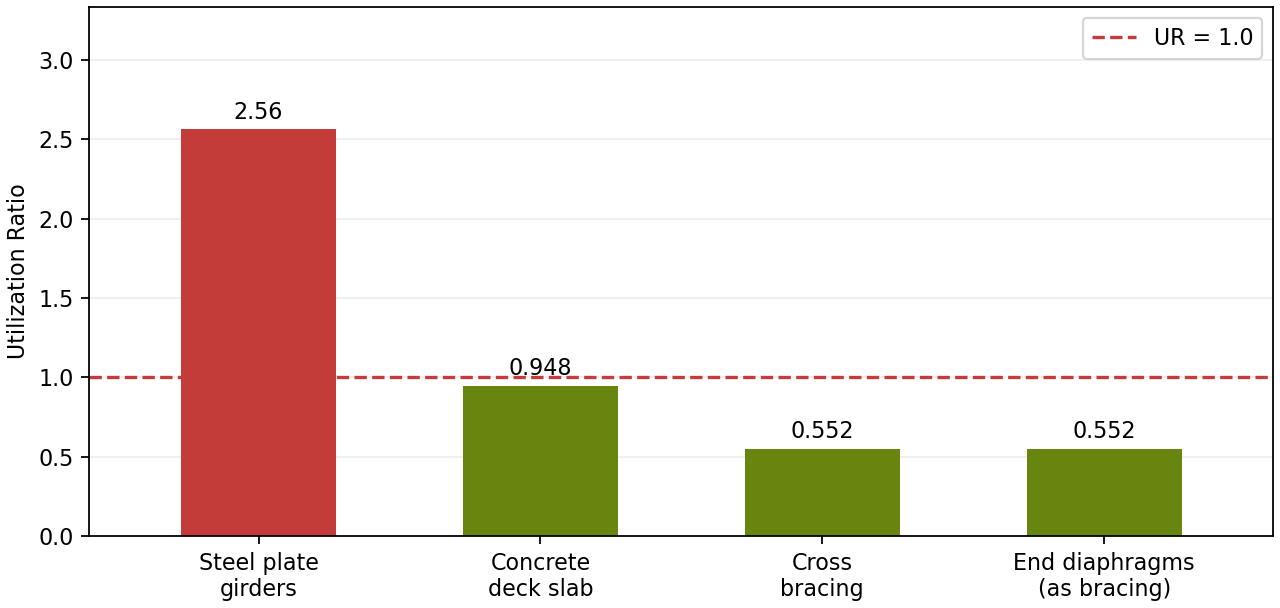
\includegraphics[width=0.94\textwidth]{Report_After_assets/utilization.png}%
\caption{Governing (maximum) utilization ratio of each primary element, taken from the checks listed in Table~\ref{tab:overall-summary}. N/A denotes unavailable design results.}%
\end{figure}
% ===========================

\ReportTableGap
\begin{longtable}{|C{3.4cm}|L{4.5cm}|C{2.3cm}|C{2.3cm}|>{\centering\arraybackslash}p{1.6cm}|}
\caption{\textbf{Overall Design Check Summary --- All Members}}\label{tab:overall-summary}\\
\hline
\textbf{Member / Check} & \textbf{Governing Load Combo} & \textbf{Demand} & \textbf{Capacity} & \textbf{UR} \\[\ReportRowGap]
\hline
\endfirsthead
\multicolumn{5}{@{}l}{\ReportContinuedFromNumbered}\\
\hline
\textbf{Member / Check} & \textbf{Governing Load Combo} & \textbf{Demand} & \textbf{Capacity} & \textbf{UR} \\[\ReportRowGap]
\hline
\endhead
\noalign{\vskip-\arrayrulewidth}\hline
\multicolumn{5}{@{}r@{}}{\ReportContinuedOn}\\
\endfoot
\endlastfoot

Girder --- Moment & ACCIDENTAL\_\allowbreak{}1:\allowbreak{} 1.0DL + 1.0DW + 0.75LL & 1341.55 kNm & 4600.16 kNm & 0.29 \\[\ReportRowGap]
\hline
Girder --- Shear & ACCIDENTAL\_\allowbreak{}1:\allowbreak{} 1.0DL + 1.0DW + 0.75LL & 303.73 kN & 550.70 kN & 0.55 \\[\ReportRowGap]
\hline
Girder --- LTB (constr.) & 1.0 DL & 705.30 kNm & 2316.41 kNm & 0.30 \\[\ReportRowGap]
\hline
Girder --- Deflection & 1.0 DL + 1.0 LL & 24.50 mm & 33.33 mm & 0.74 \\[\ReportRowGap]
\hline
Girder --- Stress & SLS\_\allowbreak{}RARE\_\allowbreak{}1:\allowbreak{} 1.0DL + 1.2DW + 1.0LL + 0.6WL & 126.05 MPa & 315.00 MPa & 0.40 \\[\ReportRowGap]
\hline
Girder --- Fatigue & SLS\_\allowbreak{}FREQUENT\_\allowbreak{}1:\allowbreak{} 1.0DL + 1.2DW + 0.75LL + 0.5WL & 237.20 MPa & 92.49 MPa & \textcolor{reportFail}{2.56} \\[\ReportRowGap]
\hline
Transverse Shear (slab) & --- & --- & --- & 0.12 \\[\ReportRowGap]
\hline
Crack Width (slab) & SLS\_\allowbreak{}FREQUENT\_\allowbreak{}1:\allowbreak{} 1.0DL + 1.2DW + 0.75LL + 0.5WL & 0.221 mm & 0.300 mm & 0.74 \\[\ReportRowGap]
\hline
Deck --- Flexure (sagging) & Basic ULS: 1.35DL + 1.5LL & 50.26 kN-m/m & 55.25 kN-m/m & 0.91 \\[\ReportRowGap]
\hline
Deck --- Flexure (hogging) & Basic ULS: 1.35DL + 1.5LL & 37.70 kN-m/m & 41.92 kN-m/m & 0.90 \\[\ReportRowGap]
\hline
Deck --- Cantilever Overhang & Basic ULS: 1.35DL + 1.5LL & 107.10 kN-m/m & 114.71 kN-m/m & 0.93 \\[\ReportRowGap]
\hline
Deck --- Punching Shear & Basic ULS: 1.35DL + 1.5LL & 0.19 MPa & 0.55 MPa & 0.34 \\[\ReportRowGap]
\hline
Deck --- One-Way Shear & Basic ULS: 1.35DL + 1.5LL & 84.75 kN/m & 107.58 kN/m & 0.79 \\[\ReportRowGap]
\hline
Deck --- SLS Stress (steel/concrete) & --- & --- & --- & 0.94 \\[\ReportRowGap]
\hline
Deck --- Min. Reinforcement (crack control) & --- & --- & --- & 0.95 \\[\ReportRowGap]
\hline
Cross Bracing --- Compression & 1.5 EQ (b) & 6.75 kN & 16.060 kN & 0.42 \\[\ReportRowGap]
\hline
Cross Bracing --- Tension & 1.5 EQ (b) & 4.95 kN & 45.000 kN & 0.11 \\[\ReportRowGap]
\hline
Cross Bracing --- Slenderness & --- & 137.9 & 250 & 0.55 \\[\ReportRowGap]
\hline
End Diaphragm --- Compression (as bracing) & 1.5 EQ (b) & 6.75 kN & 16.060 kN & 0.42 \\[\ReportRowGap]
\hline
End Diaphragm --- Tension (as bracing) & 1.5 EQ (b) & 4.95 kN & 45.000 kN & 0.11 \\[\ReportRowGap]
\hline
End Diaphragm --- Slenderness (as bracing) & --- & 137.9 & 250 & 0.55 \\[\ReportRowGap]
\hline
\end{longtable}
\noindent\textit{Note: UR = Demand / Capacity. A value $\leq 1.0$ is a passing check; values above 1.0 are shown in red. Slenderness rows give KL/r divided by its limit. A bracing-type end diaphragm is reported with the cross-bracing member results. Rows showing only a UR use the stored design ratio. The governing check for each component is highlighted in the individual design check sections above.}


\ReportSectionStyle
\chapter{Drawings and Visualizations}
\label{chap:drawings}
\noindent\textit{Drawings were not selected for this report.} Chapter numbering is kept so that the Material Take-off remains Chapter 7.

\setcounter{chapter}{6}
\ReportSectionStyle

\chapter{Material Take-off \& Quantity Summary}
\label{ch:material-takeoff}

\noindent\textbf{Table 7.1  Bill of Materials (Steel, Concrete, and Reinforcement Quantities)}

\begingroup
\ReportCompactTable
\begin{longtable}{|C{1.0cm}|L{3.8cm}|C{2.6cm}|C{1.8cm}|C{1.8cm}|C{1.8cm}|C{1.8cm}|}
\hline
\textbf{S.N.} & \textbf{Item Description} & \textbf{Volume (m$^3$)} & \textbf{Quantity} & \textbf{Total Volume (m$^3$)} & \textbf{Weight (MT)} & \textbf{Total Weight (MT)} \\
\hline
\endfirsthead
\multicolumn{7}{@{}l}{\ReportContinuedFrom}\\
\hline
\textbf{S.N.} & \textbf{Item Description} & \textbf{Volume (m$^3$)} & \textbf{Quantity} & \textbf{Total Volume (m$^3$)} & \textbf{Weight (MT)} & \textbf{Total Weight (MT)} \\
\hline
\endhead
\noalign{\vskip-\arrayrulewidth}\hline
\multicolumn{7}{@{}r@{}}{\ReportContinuedOn}\\
\endfoot
\endlastfoot

1 & Structural Steel (IS 2062) for Girders & $0.01559\text{ m}^2 \times 20.00\text{ m} = 0.31184\text{ m}^3$ & 5 & 1.56 & 2.45 & 12.24 \\
\hline
2(a) & Cross Bracing - Top Chord & $0.00024\text{ m}^2 \times 2.43\text{ m} = 0.00058\text{ m}^3$ & 24 & 0.01 & 0.0045 & 0.11 \\
\hline
2(b) & Cross Bracing - Bottom Chord & $0.00024\text{ m}^2 \times 2.43\text{ m} = 0.00058\text{ m}^3$ & 24 & 0.01 & 0.0045 & 0.11 \\
\hline
2(c) & Cross Bracing - Diagonal Chord & $0.00024\text{ m}^2 \times 2.61\text{ m} = 0.00062\text{ m}^3$ & 48 & 0.03 & 0.0049 & 0.23 \\
\hline
3 & Concrete (M40) for Deck Slab & $12.15\text{ m} \times 0.25\text{ m} \times 20.00\text{ m} = 60.75\text{ m}^3$ & 1 & 60.75 & 151.87 & 151.87 \\
\hline
4 & Reinforcement Steel (Fe 500) & $0.046433\text{ m}^2 \times 20.00\text{ m} = 0.92866\text{ m}^3$ & 1 & 0.93 & 7.29 & 7.29 \\
\hline
5 & Shear Stud Connectors & $0.000314\text{ m}^2 \times 0.100\text{ m} = 0.000031\text{ m}^3$ & 660 & 0.02 & 0.000247 & 0.163 \\
\hline
6 & Crash Barrier & $0.30228\text{ m}^2 \times 20.00\text{ m} = 6.04566\text{ m}^3$ & 2 & 12.09 & 15.11 & 30.23 \\
\hline
\end{longtable}
\endgroup
\begin{figure}[H]%
\centering%
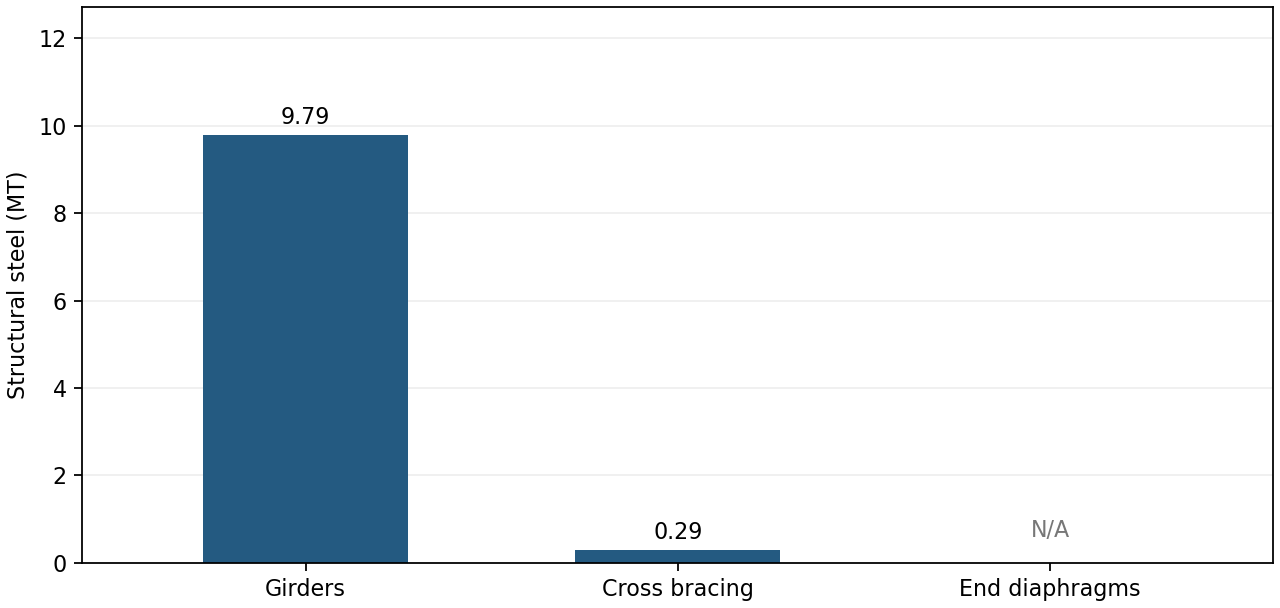
\includegraphics[width=0.94\textwidth]{Report_After_assets/structural_steel.png}%
\caption{Structural steel tonnage by component. N/A denotes unavailable quantities.}%
\end{figure}\begin{figure}[H]%
\centering%
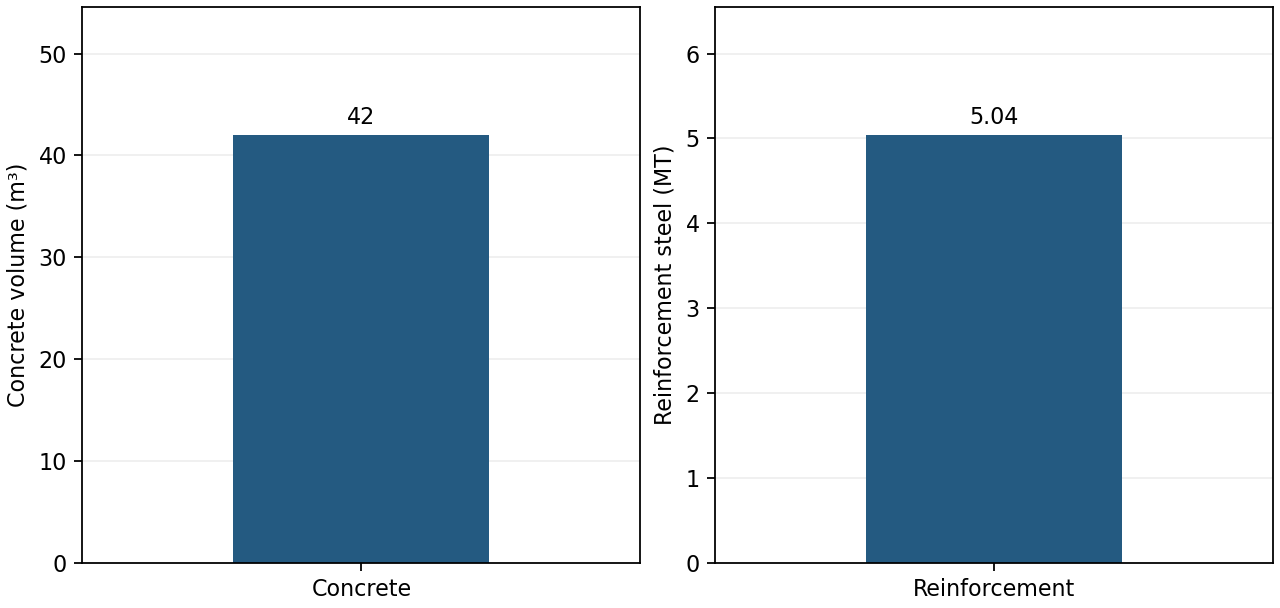
\includegraphics[width=0.94\textwidth]{Report_After_assets/concrete_reinforcement.png}%
\caption{Concrete volume and reinforcement weight on separate unit axes.}%
\end{figure}
\ReportSectionStyle

\chapter{Standards \& Assumptions}
\label{ch:Design Standards}

This section provides references to standards used to calibrate the OsdagBridge
design modules, and notes the limitations of the current software version.

\section{Design Standards}
\label{sec:design_standards}

The following Indian Road Congress (IRC) codes and Indian Standards (IS)
form the basis of all design calculations in this software.

\ReportSectionGap

\begingroup
\ReportCompactTable
\begin{longtable}{|c|c|p{12.7cm}|}

\caption{\textbf{IRC Codes}}\\
\hline
\textbf{Code} & \textbf{Year} & \textbf{Title / Scope} \\
\hline
\endfirsthead
\multicolumn{3}{@{}l}{\ReportContinuedFromNumbered}\\
\hline
\textbf{Code} & \textbf{Year} & \textbf{Title / Scope} \\
\hline
\endhead
\noalign{\vskip-\arrayrulewidth}\hline
\multicolumn{3}{@{}r@{}}{\ReportContinuedOn}\\
\endfoot
\endlastfoot

IRC 5 & 2015 & General Features of Design - carriageway widths, kerb, footpath dimensions \\
\hline
IRC 6 & 2017 & Loads and Load Combinations - dead load, live load, impact, wind, temperature, etc. \\
\hline
IRC 22 & 2015 & Composite Construction (LS) - Composite section properties, ULS/SLS design, shear connectors \\
\hline
IRC 24 & 2010 & Steel Road Bridges (LS) - Stiffener design, skew angle limits, diaphragm requirements \\
\hline
IRC 112 & 2020 & Concrete Road Bridges - Deck slab flexure, shear, crack width, reinforcement \\
\hline
IRC SP 114 & 2018 & Seismic Design of Road Bridges \\
\hline
\end{longtable}
\endgroup


\begingroup
\ReportCompactTable
\begin{longtable}{|c|c|p{12.7cm}|}

\caption{\textbf{IS Codes}}\\
\hline
\textbf{Code} & \textbf{Year} & \textbf{Scope} \\
\hline
\endfirsthead
\multicolumn{3}{@{}l}{\ReportContinuedFromNumbered}\\
\hline
\textbf{Code} & \textbf{Year} & \textbf{Scope} \\
\hline
\endhead
\noalign{\vskip-\arrayrulewidth}\hline
\multicolumn{3}{@{}r@{}}{\ReportContinuedOn}\\
\endfoot
\endlastfoot

IS 800 & 2007 & Steel construction - tension, compression, bending, shear, LTB, stiffeners, combined checks \\
\hline
IS 456 & 2000 & Concrete - simplified stress-block for deck moment capacity \\
\hline
IS 1786 & 2008 & Reinforcement steel properties \\
\hline
IS 1893 (Part 3) & 2014 & Earthquake resistant design \\
\hline
IS 2062 & 2011 & Structural steel - yield and ultimate strength by grade \\
\hline
\end{longtable}
\endgroup


\clearpage
\section{Analysis and Design Assumptions of This Version}
\label{sec:assumptions}

\textbf{Structural Analysis}

\begin{itemize}
    \item All girders are modelled as simply supported; continuous spans are not currently supported.
    \item A 3D grillage model (OSPGrillage) is used for load distribution. Grillage members carry composite section properties after the construction stage.
    \item The transverse member forces are computed using an approximate 2D frame analogy. For irregular or skewed geometries, a 3D FEM is recommended.
    \item Fixed bearing stiffness is modelled as $k = 1{,}000{,}000 \,\text{kN/m}$ (virtually rigid); free/expansion bearing as $k = 100 \, \text{kN/m}$.
    \item Construction stage sequence analysis is approximate. Detailed staged analysis should be performed for long-term deflection checks.
\end{itemize}

\textbf{Composite Action}

\begin{itemize}
    \item Full shear connection is assumed at ULS with headed stud connectors designed per IRC 22:2015 Cl.606.
    \item Short-term composite section properties (modular ratio $n = E_s/E_{cm}$) are used for ULS checks.
    \item Long-term composite section properties (with creep-adjusted modular ratio) are used for SLS deflection and crack-width checks.
    \item Pre-composite stage: the steel girder alone resists all construction loads prior to concrete gaining strength.
\end{itemize}


\textbf{Material Properties (IRC 22:2015 Annex III)}

\begin{itemize}
\item Steel: $E_s = 200{,}000 \, \text{MPa}, \ G_s = 80{,}000 \, \text{MPa}, \ \nu = 0.30, \ \alpha = 11.7 \times 10^{-6}/^\circ\mathrm{C}$ (grade-independent).
\item Minimum structural concrete grade: M25.
\item Default reinforcement grade: Fe500.
\end{itemize}

\textbf{Partial Safety Factors (IRC 22:2015 Cl.601.4)}

\begin{itemize}
\item $\gamma_{m0}$ (steel yield, ULS) = 1.10
\item $\gamma_{m1}$ (steel ultimate, ULS) = 1.25
\item Reinforcement (ULS) = 1.15
\item Welds -- shop: 1.25; field: 1.50
\item Fatigue ($\gamma_{mft}$) = 1.35
\end{itemize}

\textbf{Loading}

\begin{itemize}
\item Dead load densities per IRC 6:2017 Cl.203: structural steel $78.5 \ \text{kN/m}^3$, concrete $25.0 \ \text{kN/m}^3$, bituminous wearing course $24.0 \ \text{kN/m}^3$.
\item Multi-lane live load reduction factors per IRC 6:2017 Cl.204.4 Table 6A: 1st lane = 1.0, 2nd lane = 0.8, 3rd lane onwards = 0.4.
\item Impact factor (dynamic load allowance) computed from span per IRC 6:2017 Cl.208.2/208.3.
\item Wind load applied as transverse, longitudinal, and vertical components per IRC 6:2017 Cl.209.3.3--209.3.5.
\end{itemize}

\textbf{Serviceability Limits}

\begin{itemize}
\item Deflection limits (IRC 22:2015 Cl.604.3.2): live load + impact $\leq L/800$; total $\leq L/600$.
\item SLS stress limits: concrete $\sigma_c \leq 0.48 f_{ck}$; rebar $\sigma_s \leq 0.80 f_{yk}$; steel $f_e \leq 0.9 f_y$.
\item Permissible crack width: $w_k \leq 0.3 \ \text{mm}$ (bridge deck, exposure class XS2/XD2 per IRC 112:2020 Cl.12.3.2).
\end{itemize}

\textbf{Fatigue}

\begin{itemize}
\item Reference fatigue life: $N_{sc} = 2 \times 10^6$ cycles (IRC 22:2015 Cl.605).
\item Constant stress range is assumed. A thickness correction factor $\mu_r$ is applied for plate thickness $> 25 \ \text{mm}$.
\end{itemize}

\textbf{Stiffener Design}

\begin{itemize}
\item Intermediate transverse stiffener and bearing stiffener design follows IS 800:2007 Cl.8.7.2/8.7.3 and IRC 24:2010 Cl.509.7.2/509.7.3.
\end{itemize}


\section{Known Limitations of This Version}
\label{sec:limitations}

\begin{itemize}
\item Substructure (piers, pile caps, foundations) and bearing design are not included.
\item Splice connection design is not implemented.
\item Skew angle $>$ 15 degrees requires independent manual analysis (IRC 24 Cl. 504.8).
\item Construction stage sequence analysis is approximate; detailed staged analysis
  should be performed for long-term deflection checks.
\item The grillage analysis assumes simply supported boundary conditions;
  continuous spans are not currently supported.
\end{itemize}

\ReportSectionStyle

\chapter*{References}
\addcontentsline{toc}{chapter}{References}


\begin{enumerate}

\item IRC 5 (2024) --- \textit{Standard Specifications and Code of Practice for Road Bridges, Section I: General Features of Design.}

\item IRC 6 (2017) --- \textit{Standard Specifications and Code of Practice for Road Bridges, Section II: Loads and Load Combinations.}

\item IRC 22 (2014) --- \textit{Standard Specifications and Code of Practice for Road Bridges, Section VI: Composite Construction (Limit State Design).}

\item IRC 24 (2010) --- \textit{Standard Specifications and Code of Practice for Road Bridges, Section V: Steel Road Bridges (Limit State Method).}

\item IRC 112 (2011) --- \textit{Code of Practice for Concrete Road Bridges.}

\item IRC SP 114 (2018) --- \textit{Guidelines for Seismic Design of Road Bridges.}

\item IS 800 (2007) --- \textit{Indian Standard: General Construction in Steel --- Code of Practice.}

\item IS 2062 (2011) --- \textit{Hot Rolled Medium and High Tensile Structural Steel --- Specification.}

\item Subramanian, N. (2008). \textit{Design of Steel Structures.} Oxford University Press.

\item Steel-INSDAG Teaching Resource Materials. \url{https://www.steel-insdag.org}

\end{enumerate}

\end{document}